\documentclass[fontsize=12pt,paper=letter,twosided,cleardoublepage=plain,final]{scrbook}

\usepackage{lib/thesisformat}
\setthesisgeomery

\usepackage{lib/thesisdefinitions}

% set up bibliography
\usepackage[
  backend=bibtex,
  sortcites=true,
  sorting=ynt,
  abbreviate=false,
  style=numeric,
  citestyle=numeric,
  isbn=false,
  url=false,
  doi=false]{biblatex}
\addbibresource{bibliography.bib}

% for \begin{comment}
\usepackage{verbatim}
\usepackage{amsmath}
\usepackage{amssymb}

% for formulas
\usepackage{mathtools}

% to split lists into multiple columns
\usepackage{multicol}

% for "on page NN" reference
\usepackage[nospace]{varioref}

% for \sfrac
\usepackage{xfrac}

% for \ifoptionfinal
\usepackage{ifdraft}

% for \phantomsection
\usepackage{bookmark}
\usepackage{hyperref}

% in thesis: titlehead, subject, title, subtitle
\title{FluiDB: Adaptive storage layout using reversible relational operators}

\author{Christos Perivolaropoulos}
\date{January 2022}

\hypersetup{
    colorlinks=true,
    linkcolor=blue,
    filecolor=magenta,
    urlcolor=cyan,
    pdfpagemode=FullScreen,
    }


\begin{document}

\frontmatter
%% Start the page numbering in roman
\setcounter{page}{1}%

%% Make the title page
\maketitle%

\begin{precontent}
\dictum[Bertolt Brecht -- Life of Galileo]{ If the scientists, brought
 to heel by self-interested rulers, limit themselves to piling up
 knowledge for knowledge’s sake, then science can be crippled and your
 new machines will lead to nothing but new impositions. You may in due
 course discover all that there is to discover, and your progress will
 nonetheless be nothing but a progress away from mankind. The gap
 between you and it may one day become so wide that your cry of
 triumph at some new achievement will be echoed by a universal cry of
 horror.}
%

\chapter{Abstract}%
It is a popular practice to use materialized intermediate results to
improve performance of RDBMSes. Work in this area has focused either on
optimizers matching existing results or selecting useful intermediate
results from a plan, but few attempts have been made to create plans
with intermediate results in mind, and none that make any deduplicate
the stored data to alleviate the storage cost of maintaining possibly
large queries.

We built \emph{FluiDB} to explore a novel approach to integrating the
selection of materialized results with the planner in order to
optimize the logical representation of data in memory. FluiDB
materializes hot intermediate results and deduplucates data to
alleviate the cost of maintaining them. This is achieved by
introducing \emph{reversible operations}, versions of normal relational
operators that optionally pass enough data to the output to make the
input relations reconstructable. A planner aware of such operations
can build query plans that dynamically adapt the data layout to the
plan under constrained memory budget. This thesis revolves around four
main chapters each of which describes in detail a different part of
FluiDB and a final one that goes into evaluation of the system.

The first chapter focuses on query processing and the relational
algebra semantics that FluiDB operates under. FluiDB parses queries
into graphs of sub-queries connected by reversible operators. Each
such graph of the workload is merged into a global query graph that is
used to infer properties of each relation like cardinality and
extent.

The next chapter is dedicated to the planner and a novel monad for
weighted backtracking that the planer is based on. The planner
attempts to generate a plan based on the query graph that besides
solving the query at hand, leaves in memory an optimal set of queries
for the workload being run. In this chapter, the garbage collector is
also discussed, that creates deletion operators as part of the plan
such that the available budget is respected.

After that, we go into \emph{Antisthenis}, a novel incremental
computation system used by the query planner to determine, given a
particular set of materialized relations, whether a relation
materializable and the expected cost of materializing a
relation. Antisthenis, besides reusing computations, takes advantage
of the properties of the operations involved in the expression she is
evaluating, like absorbing group elements, to heuristically avoid as
much work as possible.

The final chapter about the FluiDB architecture describes the
transpilation of plans generated by the planner to C++, as well as the
supporting libraries that enable the evaluation of queries as C++
code, and the low level data organization of the database. The thesis
closes with a chapter that describes our methods for benchmarking and
some experimental results.

\chapter{Lay Summary}%

A database is a computer program thet can answer questions
(\emph{queries}) based on a set of data stored in a medium accessibly
by the computer running the database, as well as provides an interface
to manipulate said data. A database system will rephrase the queries
it receives in such a way that they can be answered efficiently,
breaking them down to sub-queries. A well studied method of increasing
efficiency is to store the answers to commonly encoutnered subqueries
so they are readily available. Among many other concerns that govern
the design of a database system we focus on three: deciding how to
rewrite and break down the query, inferring which subquery answers are
worth keeping around after the final answer is found, and deciding
which subquery ansers are taking up too much valuable space and should
be deleted.

This work describes the development of FluiDB, an experimental
database system that explores the idea that the three concerns in
focus are codependent and therefore could be addressed
simultenously. The design of FluiDB aspires to take one more step in
that direction by instead of allowing or evicting intermediate
results, as the probelm is traditionally conceptualized, by adapting
the very organization of the data managed by the database system to
the patterns observed by the sequence of queries.

TODO: relations between queries
TODO: antisthenis
TODO: code generation
TODO: evaluation

\chapter{Acknowledgements}%

This thesis is dedicated to all the people that directly or indirectly
supported me though my PhD studies, but also to all the people
whithout whose support and hard work I would never have started this
work to begin with.

It is customary to thank the supervisors first regardless of the
circumstances but I would like to underline my gratitude to Stratis
who really understood my idiosyncratic way of working and provided
precisely the quality and quantity of guidance that I required. This
is a rare quality and I cherish the opportunity I had to work with
him. I would also like to express my gratitude to thank Boris Grot,
not just in the general sense but because, especially during the first
years of my thesis he went out of his way to make me feel included and
gave value to my voice. For the similar reasons I would like to thank
Christophe Dubach whose door was always open and his whiteboard always
available, I deeply appreciate all the times he was willng to
patiently listen to my crazy ideas.

I would like to thank my family and especially my parents, for being
with me every step of the bumpy road that was my PhD, but mostly
because without their hard work and sacrifises a PhD would not have
been an option for me. I am priviledged and humbled and I owe it
primarily to them.

I would also like to thank Marina without whom I would definitely have
given up in one of the many moments of desparation. Thank you for
helping me with the impossible task of finishing a PhD during a
pandemic.

Special thank you to my flatmate for two years Christos Velanis who
got me safe and sound through some fairly dark times, and for the
ideological steeling brought about by this cohabitation. Thanks to him
and to Christos Maniatis for the heated philosophical debates that
would typically end after 6am.

Last but not least I would like to thank my friends that were there
though all of it, the thick and the thin Antreas, Giannis, Aisha,
Maria, Irini, Iordanis, Nelly, Christos, Pigi, Niki, The President,
and Nikolas.

%%%% DECLARATION

%% Use a custom declaration

% \declaration{I did it.}

%% Use the standard regulation declaration. Enter your
%% name for the signature line.

\standarddeclaration{Christos Perivolaropoulos}

\end{precontent}


\tableofcontents

%% List of figures
\cleardoublepage
\phantomsection
\addcontentsline{toc}{chapter}{\listfigurename}
\listoffigures
\listoflistings

\cleardoublepage%


\mainmatter

\chapter{Introduction}
\label{chapter:introduction}
\dictum[Author]{Something about the beginning of a journey.}

\begin{summary}
\item FluiDB is an in-memory RDBMs optimizes data layout for space
  efficiency w.r.t. the workload
\item The main novelty relates to the introduction of reversible
  relational operations which affords a new perspective on query
  planning and view selection.
\item She materializes all intermediate nodes and deletes garbage
  collects when she runs out of space.
\end{summary}

With the advent of technologies that make access to information
scalable and affordable, the mental and temporal gap between
collection of data and their analysis grows rapidly. At least two of
the biggest players in the the tech industry, Facebook and Google,
base their competitive advantage almost exclusively on vast amounts of
information that they have collected and their capacity for such
collection and processing. In cases like these the layout of the
stored data is independent of the growing number of applications
taking advantage of it.

A mantra in database community used to be that ``storage is cheap''
and while that is true a more complete version of the mantra might be
that ``slow storage is cheap''.

Databases have traditionally been dealing with the tradeoff between
memory and time efficiency within monetary constraints especially with
the use of intermediate result recycling technologies which employ
sophisticated ways of chosing parts of computation to be stored for
reuse. This model has had some impressive results in OLAP
workloads. We adopt a slightly different view of the problem:
executing query plans does not only leave some specific intermediate
results as residue, but rather \emph{transitions the entire storage
  state from one where the result of the query is not materialized to
  one where it is}. Whith such a notion of query planning what new
dimensions open up in the desgn space of a query planner? The creation
of FluiDB is an attempt to study some aspects of this question. In
particular FluiDB is based on the following pillars:

\begin{itemize}
\item Introduce reversible query operations that allow for more
  sophisticated plans based on available materialized views.
\item The planner itself involves a garbage collector that will delete
  materialized views or primary tables that can be materialized from
  the remaining relations.
\item An incremental numeric evaluation system allows the planner to
  efficiently and repeatedly infer the cost of materializing queries
  under a rapidly changing inventory of materialized views.
\item Query execution is based on code generation.
\end{itemize}

These concepts allow FluiDB to dynamically adapt the data layout to
the workload in ways that would not be possible in traditional
intermediate view recycling systems. To make this more concrete let's
look at an example.

Consider the following query over the TPC-H dataset that computes the
average discount per country:

\begin{code}
\begin{sqlcode}
    select      n_name, avg(l_discount)
    from        lineitem, customer, nation, order
    where       l_orderkey = o_orderkey
    and         c_custkey = o_custkey
    and         c_nationkey = n_nationkey
    and         l_shipdate > 10-11-2015
    group by    n_name
  \end{sqlcode}
\end{code}

An optimizer considering this query in isolation would come up with
some plan resembling the following following plan following:

\begin{figure}[H]
  \begin{tikzdiagram}
    \tikzset{
      every node/.style={draw,rectangle, align=center},
      sibling distance=10cm,
      level distance=3cm
    };
    \node{\gamma}
    child {node{\(\Join\)}
      child {node{\(\Join\)}
        child {node{\(\Join\)}
          child {
            node{\(\sigma_{shipdate > 10-11-2015}\)}
            child { node{lineitem}}
          }
          child {node {order}}
        }
        child {node{customer}}
      }
      child {node{nation}}
    };
  \end{tikzdiagram}
  \caption{\label{fig:single_plan}An efficient logical plan for a
    single query.}
\end{figure}

Notice how the selection (\(\sigma_{shipdate > 10-11-2015}\)) is
pushed all the way to the bottom of the tree because it is a cheap
operation (worst case a full scan over the input) and can potentially
shrink the input by a lot rendering the joins higher in the tree much
cheaper.


Consider a workload that repeatedly runs a query generated from the
following template:

\begin{sqlcode}
  select      n_name, avg(l_discount)
  from        lineitem, customer, nation, order
  where       l_orderkey = o_orderkey
  and         c_custkey = o_custkey
  and         c_nationkey = n_nationkey
  and         l_shipdate > |${min_date}|
  group by    n_name
 \end{sqlcode}


It is clear in this case that it would be beneficial if the workload
is large enough for the cost of
\(\li \Join \ord \Join \cust \Join \nation\) to be amortized
we would like to materialize the large join and only run
\(\gamma \sigma\) for each query attached as show in figure
\ref{fig:multi_plan}.

\begin{figure}[H]
  \begin{tikzdiagram}
    \tikzset{
      every node/.style={draw,rectangle, align=center},
      sibling distance=10cm,
      level distance=3cm
    };
    \node{\gamma}
    child {
      node{\(\sigma_{shipdate > \$\{min\_date\}}\)}
      child {node (mat){\(\Join\)}
        child {node{\(\Join\)}
          child {node{\(\Join\)}
            child { node{lineitem}}
            child { node {order}}
          }
          child {node{customer}}
        }
        child {node{nation}}
      }
    };
    \node[draw=none] (n) [left = of mat] {Keep materialized}
    edge [-stealth] (mat);
  \end{tikzdiagram}
  \caption{\label{fig:multi_plan}An efficient logical plan for a
    template based workload.}
\end{figure}

This shift of focus from per-query optimization to considering the
amortized cost of materialization of expensive relations is already a
tall order for most RDBMSes that feature materialized views. A simple
but effective approach to integrating incremental query
materialization and the optimization processes, was presented in
\cite{perezHistoryawareQueryOptimization}. In their approach they
maintain a \emph{history pool} (a list of all the past queries) that
is used to decide the benefit of materializing a sub-expression, and a
\emph{view pool} that keeps track of the materialized tables at every
moment. Both these sets are taken into account during planning to
produce a plan that will likely minimize the amortized cost of the
workload. After the query is planned the sets are updated. A
limitation of such an approach is that when dealing with relations
like \(\li \Join \ord\) in budget restricted settings, materialized
view storage can quickly become a scarce resource.

There is an opportunity to reduce the effect of this problem by
exploiting another common workload attribute: certain tables are
frequently subsumed by the same intermediate result. In our example
workload \(\li\) is fully subsumed by \(\li \Join \ord\), \(\li \Join
\ord \Join \cust\), and \(\li \Join \ord \Join \cust \Join
\nation\). Similarly \(\ord\), \(\cust\), and \(\nation\) are fully or
partially subsumed by these relations. It seems wasteful to always
keep the rows of all primary tables separately \emph{and} concatenated
in the rows \(\li \Join \ord \Join \cust \Join \nation\).

In particular we can retrieve the rows of \(\li\) by projecting
on the latter relation and deduplicating the resulting rows we can
obtain any of the former. In this -- contrived yet demonstrative --
example a plan taking into account amortized costs could be:

\begin{figure}[H]
\begin{minted}[escapeinside=||,mathescape=true]{trace-lexer.py:TraceLexer -x}
    Query |\(\gamma \sigma_{p_0}(\li \Join \ord \Join \cust \Join \nation)\)| {
      |\(Q_0\)| := Materialize[|\(\li \Join \ord\)|]
      |\(Q_1\)| := Materialize[|\(\cust \Join Q_0\)|]
      |\(Q_2\)| := Materialize[|\(\nation \Join Q_1\)|]
      # Not enough space to continue. Delete relations that we can rebuild.
      GC {
        Delete[|\(\li\)|]
        Delete[|\(Q_0\)|]
      }
      |\(Q_3\)| := Materialize[|\(\sigma_{p_0} Q_2\)|]
      |\(Q_4\)| := Materialize[|\(\gamma Q_3\)|]
    }
    Query |\(\gamma \sigma_{p_1}(\li \Join \ord \Join \cust \Join \nation)\)| {
      GC {
        Delete[|\(Q_1\)|]
      }
      |\(Q_5\)| := Materialize[|\(\sigma_{p_1} Q_2\)|]
      |\(Q_6\)| := Materialize[|\(\gamma Q_5\)|]
    }
    Query |\(\gamma \sigma_{p_2}(\li \Join \ord \Join \cust \Join \nation)\)| {
       GC {
        Delete[|\(\cust\)|]
       }
      |\(Q_7\)| := Materialize[|\(\sigma_{p_2} Q_2\)|]
      |\(Q_8\)| := Materialize[|\(\gamma Q_7\)|]
    }
    ...
    # Since the large join has all the columns of \li we should be able
    # to create it by simply getting slicing and deduplicating
    Query |\(\li\)| {
      |\(\li\)| := Materialize[|\(uniq\{\pi_{cols(\li)} Q_2\}\)|]
    }
\end{minted}
  \caption{\label{fig:amortized_plan}A sequence of plans optimizing
    the workload amortized cost and involving reverse
    operations. These queries are the same save for the predicate
    \(p_i\) selecting \(\li\)}
\end{figure}

By incorporating reverse relational operations where possible FluiDB
can indeed generate workload plans similar to the one described.

The solution we experiment with by implementing FluiDB resembles the
solution provided in \cite{gouSupSearchEfficient2006} by Gou et.al for
multi-quer. In their work they embed aggregations \sql{group by x1,
  .., xk} into the \(\subseteq\)-lattice that arises from the powerset
\(P(\{x_1, ..., x_k\})\). Thereby they encode the fact that \sql{group
  by A, B, C} is subsumed, or can be computed by, either of \sql{group
  by A, B}, \sql{group by A, C} or \sql{group by B, C}. Once the
lattice is constructed a variant of the \(A^{\star}\) path finding is
used algorithm to search for the optimal aggregation plan. However
they make no attempt to recycle tables, ie. garbage collect tables,
whose data can be found in other relations, and narrows it's attention
to aggregations.


% TODO: rewrite: we are like
% \cite{mistryMaterializedViewSelection2001} AND-OR but
%
% - bidirectional
% - not only aggregations
% - out contains complements
% - Interleave GC when traversing
From the aforementioned work we keep the basic notion of using a graph
to represent relationships between queries and to derive the benefit
of materializing a relation. We also use path finding techniques in
that graph to create plans. However we introduce a more complex and
ad-hoc hierarchy of relations to account for subsumptions the entire
relational algebra, rather than just aggregations. That is very
similar to AND-OR dags as found in
\cite{mistryMaterializedViewSelection2001}.  Furthermore the relations
we express in that graph are bidirectional. So rather than only
finding paths towards the goal and deleting relations when they are no
longer needed, we simultaneously plan for moving towards the goal
query and performing "backwards" operations for saving up space. We
clarify this with an example which demonstrates a slightly simplified
version of our system's functionality.

In figure \ref{fig:intro_selectexample} we provide representation of a
subsumption graph that our RDBMS might create after witnessing
selections on \(\li\). For brevity let \(p:=shipdate > 10-11-2015\),
\(q:=quantity < 24\) and \(r:=discount < .06\). The RDBMS has
encountered \(\sigma_{p}(\li)\), \(\sigma_{q}(\li)\) and \(\sigma_{q}
\sigma_{r} (\li)\).


\begin{figure}[H]
  \begin{tikzdiagram}
    \tikzset{
      grow=up,
      sibling distance=10cm,
      level distance=3cm,
      every node/.style={draw},
      mat/.style={fill=gray!30}
    };

    \newcommand{\n}[1]{node {\(#1\)}}
    \newcommand{\bn}[1]{node[mat] {\(#1\)}}

    \node {\(\li\)} % \li
    child { \bn{\sigma_{q}(\li)}} % σ_q
    child { \bn{\sigma_{\neg q}(\li)}} % σ_nq
    child { \n{\sigma_{\neg p}(\li)}}  % σ_np
    child {
      \n{\sigma_{p}(\li)} % σ_p
      child {\n{\sigma_{p \land r}(\li)} } % σ_pq
      child {\n{\sigma_{p \land \neg r}(\li) }} % σ_rpq
    } ;
\end{tikzdiagram}
\caption{\label{fig:intro_selectexample}The materialized relations are
  marked with grey. Assuming the absense of null values and assuming
  set semantics
  \(\li = \sigma_p \li \cup \sigma_{\neg p} \li\).
  FluiDB can find a plan to generate any of the relations in the graph
  from \(\sigma_p \li\) and \(\sigma_{\neg p} \li\).  }
\end{figure}

% TODO: Benefit order: \sigma_q > \sigma_{p \land r} > \sigma_p >
% \sigma_{\neg q} > ... > \li.

The query that we are planning is \(\sigma_{quantity < 24}
\sigma_{discount < .06} (\li)\), which is denoted in the figure as
\(\sigma_{q \land r}(\li)\). Our total size budget is 2.5.

Following the edges in the graph, to plan \(\sigma_{q \land r}(\li)\)
we need \(\sigma_{q}(\li)\) and for that we need \(\li\) and is least
beneficial. So first we plan the union

\[
  \sigma_{\neg p}(\li) \cup \sigma_{p}(\li) \rightarrow \li
\]

Then we need \(\sigma_{q}(\li)\) but we are now using 2 units of space
and adding .6 more would exceed our space budget of 2.5. \(\li\) is
the least beneficial of our materialized views but it is required for
our next step, ie. creating \(\sigma_{q}(\li)\) . \(\sigma_{\neg
p}(\li)\) is deleted since it's derivable from \(\li\). Then
\(\sigma_{q}(\li)\) is created and now we are using 2.1 units of
space.

\[
  \li \rightarrow \sigma_{q}(\li)
\]

Finally we need to create the final relation \(\sigma_{q \land
  r}(\li)\) . However it's space requirement is .5 and we we would
be exceeding our budget. We can't delete \(\li\) even though it
is our least beneficial table because we would have no way of
recreating it.

Here we have two options. One is to delete \(\sigma_{\neg
  p}(\li)\), our most benefit al table. The other, which is the one
that the system should opt for, is to backtrack. When we created
\(\sigma_{q}(\li)\), instead we create both
\(\sigma_{q}(\li)\) and \(\sigma_{\neg q}(\li)\).

\[
  \li \rightarrow \{\sigma_{q}(\li), \sigma_{\neg q}(\li)\}
\]

Once both those tables are materialized we can safely delete
\(\li\). Now our space usage is 1.1 and we can safely

\[
  \sigma_{q}(\li) \rightarrow \sigma_{q \land r} (\li)
\]

Which is the requested query and, in summary, the final can be
represented as:


\begin{figure}[H]
\begin{minted}[escapeinside=||,mathescape=true]{trace-lexer.py:TraceLexer -x}
    Inventory {
      |\(Q_0\)| := |\(\sigma_{\neg p}(\li)\)|
      |\(Q_1\)| := |\(\sigma_{p}(\li)\)|
      ...
    }
    Query |\(\sigma_{q \land r} \mathit{\li}\)| {
      |\(\li\)| := Materialize[|\(Q_0 \cup  Q_1\)|]
      GC { Delete[|\(Q_0\)|] }
      |\(Q_2\)|,|\(Q_3\)| := Materialize[|\(\{\sigma_{q}(\li), \sigma_{\neg q}(\li)\}\)|]
      GC { Delete[|\(\li\)|] }
      |\(Q_4\)| := Materialize[|\(\sigma_{r} Q_2\)|]
    }
\end{minted}
  \caption{\label{fig:reverse_operations}A sequence of plans optimizing
    the workload amortized cost and involving reverse operations.}
\end{figure}

% TODO: Paragraph: contenxt where it is important to strictluy manage
% space: in-memory database. In that vain fluidb makes heavy use of of
% code generation.

% TODO: Chapter titles.
This thesis describes in detail how we implemented a system targeted
at performing this kind of reasoning to planning and executing
queries. In chapter \ref{chapter:background} we provide a brief
overview of the state of the art and common practices that pretain to
query processing; in chapter \ref{chapter:fluidb_logical_planning} we
describe how queries are processed and stored at a logical level; in
chapter \ref{chapter:physical_planning} we describe how FluiDB
performs planning and garbage collection to come up with a concrete
physical plan for each query; in chapter
\ref{chapter:execution_engine} we go over the algorithms and
particular techniques that FluiDB employs to transpile the physical
plan into C++ code; finally at chapter \ref{chapter:evaluation} we
describe our exprimental evaluation of FluiDB on the benchmark
SSB-TPC-H. We present a conclusion and some future directions in the
final chapter \ref{chapter:conclusion}


\chapter{Background}
\label{chapter:background}

FluiDB is a system that focuses on relational query processing. This
chapter aims to give the reader some idea about where FluiDB fits in
the design space and the historical context in which it was developed.
First we outline a very high level overview of the query language and
operators involved in database management, as well as the the overall
architecture of such systems. Following that we will focus on the
query processing subsystems of relational query databases and some
traditional approaches to query evaluation. Afterwards we will focus
particularly on in-memory relational databases and the tradeoffs that
govern their design. Finally we look into systems that utilize
intermediate result recycling and how they solve the problem of
automatically selecting and maintaining intermediate results for
workloads.

\section{Background: relational databases}
\label{sec:org5af5e27}
Databases are more than just a method of accessing data. In their
essence they are machines for question answering. The typical database
works in a prepetual loop of reading queries and coming up with
answers based on a set of datapoints. There are two important aspects
that every database needs to define in order to delineate its
operational semantics:

\begin{itemize}
\item The language in which the queries are expressed in
\item The representation of data in terms of which the queries are
expressed and the results are presented.
\end{itemize}

The oldest, most studied and most common model is the relational model
which defines queries in terms of \emph{relational algebra} and organizes
data in \emph{tables} or relations.

A relation is typically an unordered set of tuples
\((d_1,d_2,...,d_k)\) where each element \(d_i\) represents an
attribute. The core relational algebra is an extension of the algabra
of set (that defines operators of set union \(\cup\), intersection
\(\cap\), product \(\times\), and difference \(-\)) that includes the
operators of joins \(\Join\), projection \(\pi\) and selection
\(\sigma\). Upon this foundation relational databases typically define
extra operators to increase the expressive power of the language like
aggregations \(\gamma\), semijoins \(\lsemi\), sorting, limiting, etc.

A typical relational database processes operates in a cascading
fashion. It initially receives a query in textual form. While
relational algebra is the language that underpins the operation of a
relational database it is raraly the language in which users interact
with it. Instead, most relational databases expect queries writen in a
variant of SQL, a query language that is parsed and immediately
translated to a tree of relational algebra operators.

This tree is processed by the query optimizer which rewrites it into a
representation that is efficitent to be executed by taking advantage
of the mathematical properties of RA and often gathered statistics
about the underlying data itself. This process leads to the formation
of a relational algebra expression called the \emph{logical plan}. It is a
high level recipe of what logical operators would produce the
requested result.


Each RA operator is typically implemented by several different
algorithms, each being efficient and even possible in some situations
but not in others. For example a join can be implemented by nested
loops or with merge join.  While the former algorithm is general and
can implement any join, it is very inefficient. On the other hand a
merge join is much more efficient but can only implement joins of the
form \(\Join_{a=b}\) (equijoins). Furhtermore a logical plan typically
contains only implied information about the scheduling of the
operators, for example the logical plan \((\pi A) \Join (\sigma B)\)
implies that the join can not begin being evaluated before the
projection and the selection but the latter can be evaluated in any
order. All these details about the execution of the query are resolved
by the \emph{physical planner}. The physical planner accepts a logical
plan and emits an unambiguous sequence of steps that will produce the
result of the query.

The final step is actually executing the physical plan which is
handled by the \emph{query execution engine}. The execution engine simply
evaluates the physical plan on top of the data, making use of the
correct algorithms, auxiliary structures like indexes managing memory,
handling page-level caching, etc.

\section{Background: query processing}
\label{sec:org1ddf14b}
Query optimization and more generally query processing and planning
refer to the processes that take place between reading a query and
computing a physical plan. The concerns of query processing are
correcness of the final result and the efficiency of the plan
generated, usually in terms of time, but also in terms of space.

Finding an optimal plan is in the general case NP-complete
\cite{ullmanInformationIntegrationUsing1997}, but query optimizers can
do a good job at finding good plans using heuristics. The selection
and organization of these heuristics as well as query cost estimation
are the main problems that make a query optimizer non-trivial. In
particular there one could separate the the tasks of a query optimizer
into three broad categories:

\begin{itemize}
\item Query rewriting
\item Query plan enumeration
\item Size and cost estimation (cost model)
\end{itemize}

At a very high level the architecture of a query optimizer is
demonstrated in figure \ref{fig:org171f336} and is broadly
comprised of the following components:

\begin{figure}[p]
\centering
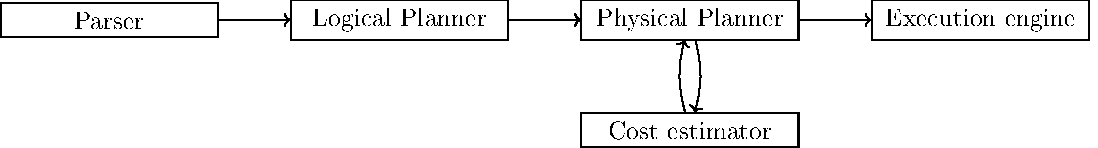
\includegraphics[width=\textwidth]{./imgs/optimizer_architecture.pdf}
\caption{\label{fig:org171f336}Common architecture of a query optimizer.}
\end{figure}

\begin{itemize}
\item The \emph{parser} which receives the query in textual form and produces a
logical plan in the form of an abstract syntax tree.
\item The \emph{deterministic optimizer} or \emph{logical planner} that rewrites the
logical plan applying optimization that are based solely on the
general properties of the relational algebra.
\item The \emph{physical planner} that transforms a logical plan into a
physical plan that can be unambiguously executed by the execution
engine to produce a result. The physical planner typically has at
least some information about the underlying data that the plan will
operate on like estimations about the statistics of the values or
the cardinalities of the relations.
\item The information about the data being manipulated by the plan is
inferred by the \emph{cost estimator}. It uses a cost model to predict
the cost of plans and cardinality of relations by taking into
account the provenance of relations as well as physical properties
of the data like presence of indexes, the data layout, etc.
\end{itemize}

These subsystems are presented here as separate for simplicity and
because in many database systems they are clearly delineated but it is
also common that they blur into each other. For example in some RDBMSs
the physical and logical planner are merged into one
\cite{graefeCascadesFrameworkQuery1995,shankarQueryOptimizationMicrosoft2012,solimanOrcaModularQuery2014}. In
fact, it is more and more common for systems to intersperse query
planning with query execution, adapting the optimization strategy
\cite{graefeDynamicQueryEvaluation1989} to concrete information about
the intermediate results evaluated rather than purely relying on
estimations and predictions
\cite{dingPlanStitchHarnessing2018,chaudhuriPayasyougoFrameworkQuery2008,wuSamplingbasedQueryReoptimization2016,herodotouXplusSqltuningawareQuery2010}. The
degree to which these subsystems are separate is a major concern in
the desgin space of query optimizers.

Another important concern to be considered, and which is indeed is
important in the design of FluiDB, is the number of queries considered
at a time during optimization and the way in which they are
considered. The optimizer usually considers one query at a time and
maintains little or no state between executions. For a very long time,
however muti-query optimization has been researched
\cite{michiardiCachebasedMultiqueryOptimization2021,wangMultiqueryOptimizationMapreduce2013,royEfficientExtensibleAlgorithms2000,rogersMultiqueryOptimization2017}
although no mainstream databases. What is more common in recent years
is recycling intermediate results. These RDBMSs materialize and cache
intermediate relations in the hopes that they will be useful for reuse
in later queries
\cite{perezHistoryawareQueryOptimization2014,nagelRecyclingPipelinedQuery2013,ivanovaArchitectureRecyclingIntermediates2010}.

The final concern that is relevant to the design of FluiDB regards the
traversal and pruning of the search space. As mentioned, query
optimization is generally NP-complete, so the viable options DBMS
designers are left with are randomized algorithms, ML approaches, and
heuristics. Virtually all systems implement heuristics entirely or to
some degree, while more and more incorporate randomized algorithms
\cite{chandeGeneticOptimizationJoin2011} and machine learning
\cite{liMachineLearningDatabases2021,marcusNeoLearnedQuery2019}.

\subsection{Logical and physical query optimization}
\label{sec:org86152ae}

The logical planner accepts a syntax tree in the form of relational
algebra where the operators only contain information about the
semantic meaning of operations and none relating to the algorithms
that will eventually be executed or the input data. It is for all
intents and purposes a rewrite engine for relational algebra. Typical
transformations performed by the logical query optimizer are

\begin{itemize}
\item Predicate normalization to conjunctive normal form, e.g. \((a_0 = 1
  \land a_1 = b_1) \lor b_2 = 3 \hookrightarrow (a_0 = 1 \lor b_2 = 3)
  \land (a_1 = b_1 \lor b_2 = 3)\)
\item Predicate pushdown e.g. \(A \Join_{a_0 = 1 \land p} B
  \hookrightarrow (\sigma_{a_0 = 1} A) \Join_p B\).
\item Cartesian products to joins \(\sigma_p ( A \times B )
  \hookrightarrow A \Join_p B\)
\item Searching the join ordering space.
\end{itemize}

Physical query planner, on the other hand, will specialize the logical
operators deciding on the particular algorithm that should be used. A
physical query planner therefore requires low level information about
the query that relates to indexes available, possible ordering of the
data, materialized views, etc.

Either of the planners needs to enumerate the plans under
consideration while traversing the search space. There are two major
approaches to this:

\begin{itemize}
\item The \emph{top-down} approach, where the planner establishes the top level
operator and branches searching the children, backtracking as
necessary. This was the approach of the decendants of the volcano
\cite{graefeVolcanoOptimizerGenerator1993a} where they implement a
"seach engine" that uses a branch and bound approach to optimization
with caching.
\item The \emph{bottom-up} approach where the builds and connects fragments of
a plan
\cite{raasveldtDuckdbEmbeddableAnalytical2019,kemperHyPerHybridOLTP2011}
\end{itemize}

An important optimizer, on which most modern optimizers are still
being based, is the cascades optimizer
\cite{graefeCascadesFrameworkQuery1995}. In short, cascades keeps track
of \emph{groups} of equivalent expressions of queries and uses those as the
fundamental atom that it manipulates. For example instead of keeping
track of \(A \Join (B \Join C)\) and \((A \Join B) \Join C\)
separately they would be part of the same query group. It then uses a
global hash table (the "memo" structure) to match the best plan that
corresponds to each group.

Many database systems use optimizers similar to cascades (like the
Microsoft SQL server, postgres, and
MemSQL\cite{chenMemSQLQueryOptimizer2016}, and greenplum -- now orca
\cite{solimanOrcaModularQuery2014a} to name a few). Notable among them
is apacha calcite \cite{begoliApacheCalciteFoundational2018}, a
framework for implementing query processing used by a number of
commercial and research databases
\cite{nunesalonsoBuildingPolyglotData2020}.

\subsection{Cost estimation}
\label{sec:org4f8e111}

Probably the hardest aspect of the planner design is the cost
estimation algorithms. These are required in order to select plans a
and to navigate the search space. A good cost model can help basic
planners make decent plans and sophisticated planners make horrible
plans \cite{leisHowGoodAre2015} . As cost estimation we refer to a
number of different related procedures that are broadly the estimation
of the cost of an arbitrary plan and include the prediction of the
cardinality of not yet materialized relations.

It seems that the most important challenges involved in the design of
a cost model is that we are fundamentally operating with scares with
scarce and highly uncertain information. Especially relating to
cardinality estimation, the most important of the tasks involved,
uncertainty and bad predictions propagate and make make it extremely
hard for the planers to make correct decisions. Consider for example a
join. Some joins are similar to cartesian products, producing large
output tables, and some joins are more similar to lookups producing
only a few rows. A cost model that confuses the kind of join will make
very bad predictions w.r.t. the cost of any relational algebra
expression that uses said join. Therefore join order estimation, that
is a critical aspect of planning.

Cost estimation is beyond the scope of FluiDB and we only implement
the most naive cardinality estimation but it is worth mentioning how
more mature systems approach the issue. Cardinality estimation most
commonly takes the form of selectivity estimation, i.e. what
percentage of tuples from the input make it to the output of a
selection or a join. This is sensitive to the statistical
properties of the values and the selection/join predicates.

The most common approach to this issue is to maintain pre-computed
statistics relating to the primary tables. This is much better than
keeping no stats but they are very hard to maintain and their
effectiveness becomes very limited for complex queries. Another
approach employed is to delay the decisions of the optimizer and
essentially merge the panner with the execution engine. This does not
completely eliminate the problem but it allows the system to have more
up to date and precise data that would allow it to correct cource
early in the event of exceptionally bad estimations. One family of
techniques that is becoming popular and was initially used in IBM DB2
\cite{stillgerLEODB2LearningOptimizer2001}, is caching the statistics
of previously computed relations and use that data to make better
predictions in the future. More recently this takes the form of
employing machine learning to learn from past cardinalities
\cite{ortizEmpiricalAnalysisDeep2019}.

To give the reader a more well rounded intuition of the state of cost
estimation besides cardinality estimation it is worth mentioning that,
to estimate the cost of an operatior, postgres uses magic configurable
variables to weigh IO with CPU evaluation time, while DB2 runs
microbenchmarks on the production system to make these estimations.


\section{Background: in-memory relational databases}
\label{sec:org96af629}
In-memory databases are databases where all the data lives in main
memory. The design of in-memory databases is different from the desgn
of a disk-backed database in a number of respects. To name a few:

\begin{itemize}
\item Page buffers have no use and caching of data in general has very
different goals. While in disk databases caches are mainly used to
avoid disk IO, in memory databases they focus on short-circuiting
computation.
\item Concurrency control is much simpler as storage synchronization
concerns are almost entirely eliminated.
\item In disk backed databases only a small percentage of time is spend on
actual computation \cite{harizopoulosOLTPLookingGlass2018}. Much of
the non-compute latency is directly linked to the persintent
storage.
\end{itemize}

On the other hand there are concerns that are specific to the lack of
backing database storage. A few of those are:

\begin{itemize}
\item Should the system rely on record IDs like in a persistent database
or can it use direct pointers to records?
\item Error prone software can bring the data to an irrecoverable state.
\item Query execution algorithms have fundamentally different
charadteristics. While in persistent databases IO dominates the
runtime the bottlenecks for an in-memory database are much more
complex and they can include things like locking, cache misses,
predicate evaluation data movements.
\item As main memory is a much less abundant resourse than presistent
storage, in-memory databases are often distributed making network a
major concern.
\end{itemize}

One increasingly common technique to address many of these issues,
which is also used by FluiDB, is \textbf{code generation}. Since workloads
for in-memory databases are typically CPU bound, there are major gains
in performance to be had by specializing the code being executed. The
typical generic code being run makes heavy use of virtual function
calls and conditionals inside tight loops which kills performance on
virtually all modern architectures. The value proposition of code
generation is to inline or hardcode the virtual functions and erase
the conditionals at runtime to reduce the number of operations and
make better use of hardware optimizations.

We identify 4 different approaches in the literature to solving this
problem:

\subsection{Transpilation}
\label{sec:orgbf8a953}

Transpilation of a physical plan to a systems language like C or C++
which is then fed to an off the shelf compiler
\cite{krikellasGeneratingCodeHolistic2010}. This approach is expensive
but it generates highly efficient code more easily debuggable
execution plans. The most notable complete database system that used
this technique is Microsoft Hekaton that generates C code and some
older versions of MemSQL. For FluiDB we reuse a lot of techiques
introduced in HIQUE \cite{krikellasGeneratingCodeHolistic2010} to
translate physical plans to template-heavy C++ code, making the
assumption that query compilation will be much faster than the query
runtime.

\subsection{Thrid party compilers}
\label{sec:orgdf395cd}

JIT compilation has received a lot of attention in the compiler
community, especially in the context of the JVM. A number of database
systems have taken advantage of this to speed up query execution. Most
notable of these are SPARK \cite{armbrustSparkSQLRelational2015}, which
generates scala AST which is then converted to JVM byte code, and
Neo4j that directly generates bytecode out of the queries.

Systems like Peloton \cite{menonRelaxedOperatorFusion2017} and recently
postgres \cite{sharyginQueryCompilationPostgreSQL2017} compile query
plans to LLVM IR code that is then fed to the LLVM compiler to
generate high performance machine code. Notable among the systems that
use this approach is HyPer \cite{neumannEvolutionCompilingQueryEngine}
which addresses the problem of the query compilation overhead with an
adaptive execution apprach: they built an IR interpreter that starts
running the query while the compiler does proper compilation of the
LLVM IR program being interpreted. Cheap queries are thus completed
reasonably fast while in the case of complex queries the interpreted
program is seamlessly replaced by the compiled one once the LLVM
compiler finishes generating machine code.

\subsection{Direct machine code generation}
\label{sec:org344a12c}

Some databases do not reuse any compiler or JIT-ing VM, but rather
directly generate highly specific machine code out of the physical
plan. The first system to attempt that, like most techniques used
today, was System R which originally compiled SQL statements directly
to machine code by stitching together code fragments from a fragment
library \cite{chamberlinHistoryEvaluationSystem1981} but it was quickly
deprecated due to the large engineering effort required. Oracle [ref]
also includes similar to some of their databases and MemSQL express
their plans in a custom language called MPL (MemSQL Plan Language) for
which they have a custom compiler that translates it directly to
machine code.

\subsection{Custom execution engines}
\label{sec:org7bca3a3}

TODO: read these papers a bit more carefully

A final category is per-database code generation rather than per-query
code generation. Volcano/EXODUS
\cite{graefeVolcanoOptimizerGenerator1993a} and more recently SageDB
\cite{kraskaSageDBLearnedDatabase} generate the optimizer and execution
engine that is specific to the database schema but not to the queries.


\section{Background: intermediate result recycling}
\label{sec:org1a32ec6}
A materialized view is a relation defined by a query that is
persistently stored. A view that is not stored is said to be
virtual. \textbf{View selection} is the process of selecting an apropritate
set of materialized views to imporve the performance of a workload
\cite{mamiSurveyViewSelection2012}.  Automated materialized view
selection or intermediate view recycling has been on the radar of the
database research community for a while now. A few approaches to this
problem have to do with AND/OR directed acyclic graphs
\cite{guptaSelectionViewsMaterialize1997}, modeling the problem as a
state optimization \cite{theodoratosDataWarehouseConfiguration1997},
and lattices to represent data cube operations (i.e. multiple
aggregations over the same relation) \cite{ImplementingDataCubes}.

A related problem is multi-query optimization
\cite{theodoratosDataWarehouseConfiguration1997} that attempts to plan
multiple queries simultaneously. An efficient solution using AND/OR
DAGs was proposed by Roy in \cite{royEfficientExtensibleAlgorithms2000}
where they insert queries and their subqueries in a graph and attempt
to evaluate a plan by traversing that graph from multiple sources in a
fashion similar to volcano optimization. Building on that Kathuria
et. al. prresent an approximation algorithm that runs in time
quadratic to the number of common subexpressions and provides
theoretical guarantees on the quality of the solution obtained
\cite{kathuriaEfficientProvableMultiquery2017}.

Researchers have further looked at opportunistically reusing
intermediate results that would be materialized
\cite{ivanovaArchitectureRecyclingIntermediates2010,nagelRecyclingPipelinedQuery2013}. It
has been researched in non-strictly database contexts like MapReduce
\cite{elghandourReStoreReusingResults2012a}, and there have been
attempts to unify the planner with the materialized view selection
engine \cite{perezHistoryawareQueryOptimization2014a}. Notable in this
field is Nectar \cite{gundaNectarAutomaticManagement2010} which is also
not an RDBMs. It automatically compresses rarely used data into
programs that generate that data. Nectar focuses on sharing
computation and data as much as possible.

Work such as MRShare \cite{nykielMRShareSharingMultiple2010} tries to
bridge the gap betweem intermediate result recycling and MQO by
automatically grouping queries in a workload in such a way that
computation can be maximally shared.


\chapter{Logical planning}
\label{chapter:fluidb_logical_planning}
\begin{frame}
  \frametitle{Logical planning}
  \begin{itemize}
  \item Bipartite query graph -- RA operations/relations unified for all queries
  \item Join ordering enumeration
  \item QNF -- \(\pi \sigma (Q_1 \times Q_2 \times \dots )\) or
    \(\gamma \sigma (Q_1 \times Q_2 \times \dots )\)
  \item Relation shape propagation -- cardinality, columns/types, unique subtuples
  \end{itemize}

\end{frame}

\begin{frame}
  \frametitle{Reversible operators}
  \begin{columns}
    \begin{column}{0.5\textwidth}
      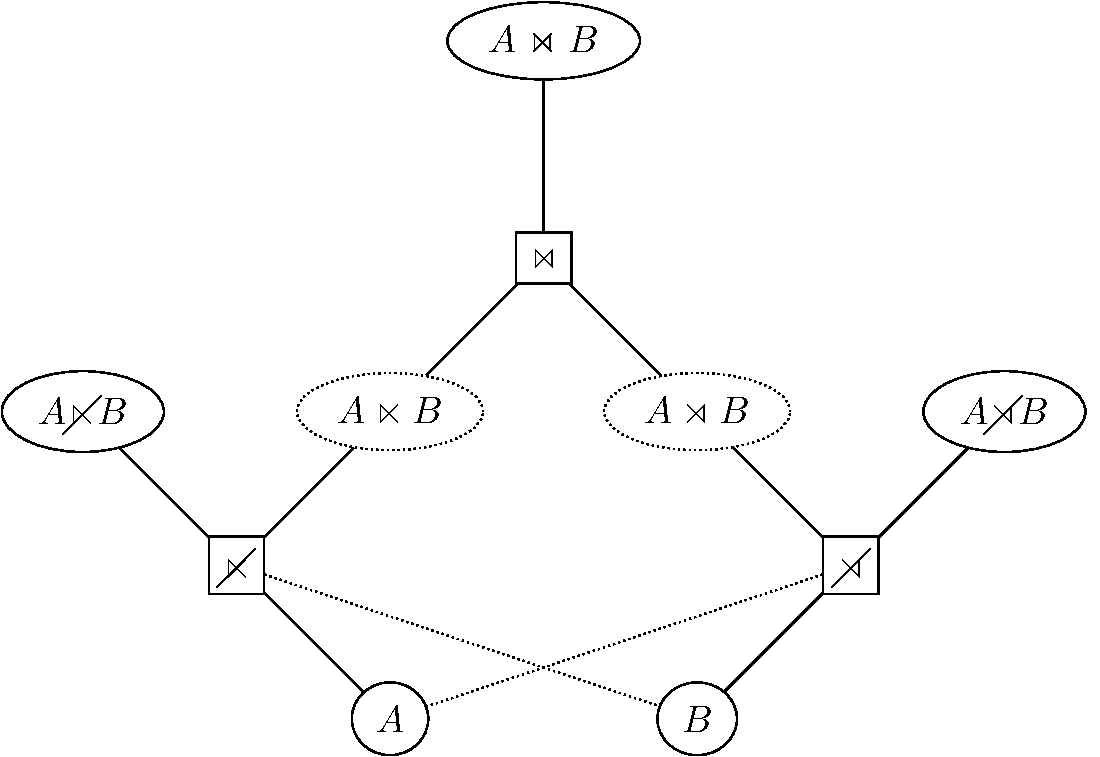
\includegraphics[width=.9\linewidth]{../imgs/joinnet.pdf}
   \end{column}
    \begin{column}{0.5\textwidth}
      \begin{tikzdiagram_w}
        \tikzset{node distance=2cm}
        \tikzset{nnode/.style={ellipse,draw}}
        \tikzset{tnode/.style={rectangle,draw}}

        \node[tnode] (t) {\(\sigma_p\)};
        \node[nnode] (o2) [above left of=t] {\(o_{sec}\)};
        \node[nnode] (o1) [above right of=t] {\(o_{prim}\)};
        \node[nnode] (i) [below of=t] {\(i\)};

        \path (t) edge (i);
        \path (t) edge (o1);
        \path (t) edge (o2);
      \end{tikzdiagram_w}
    \end{column}
  \end{columns}
\end{frame}

\begin{frame}
  \frametitle{Reversible operations}
  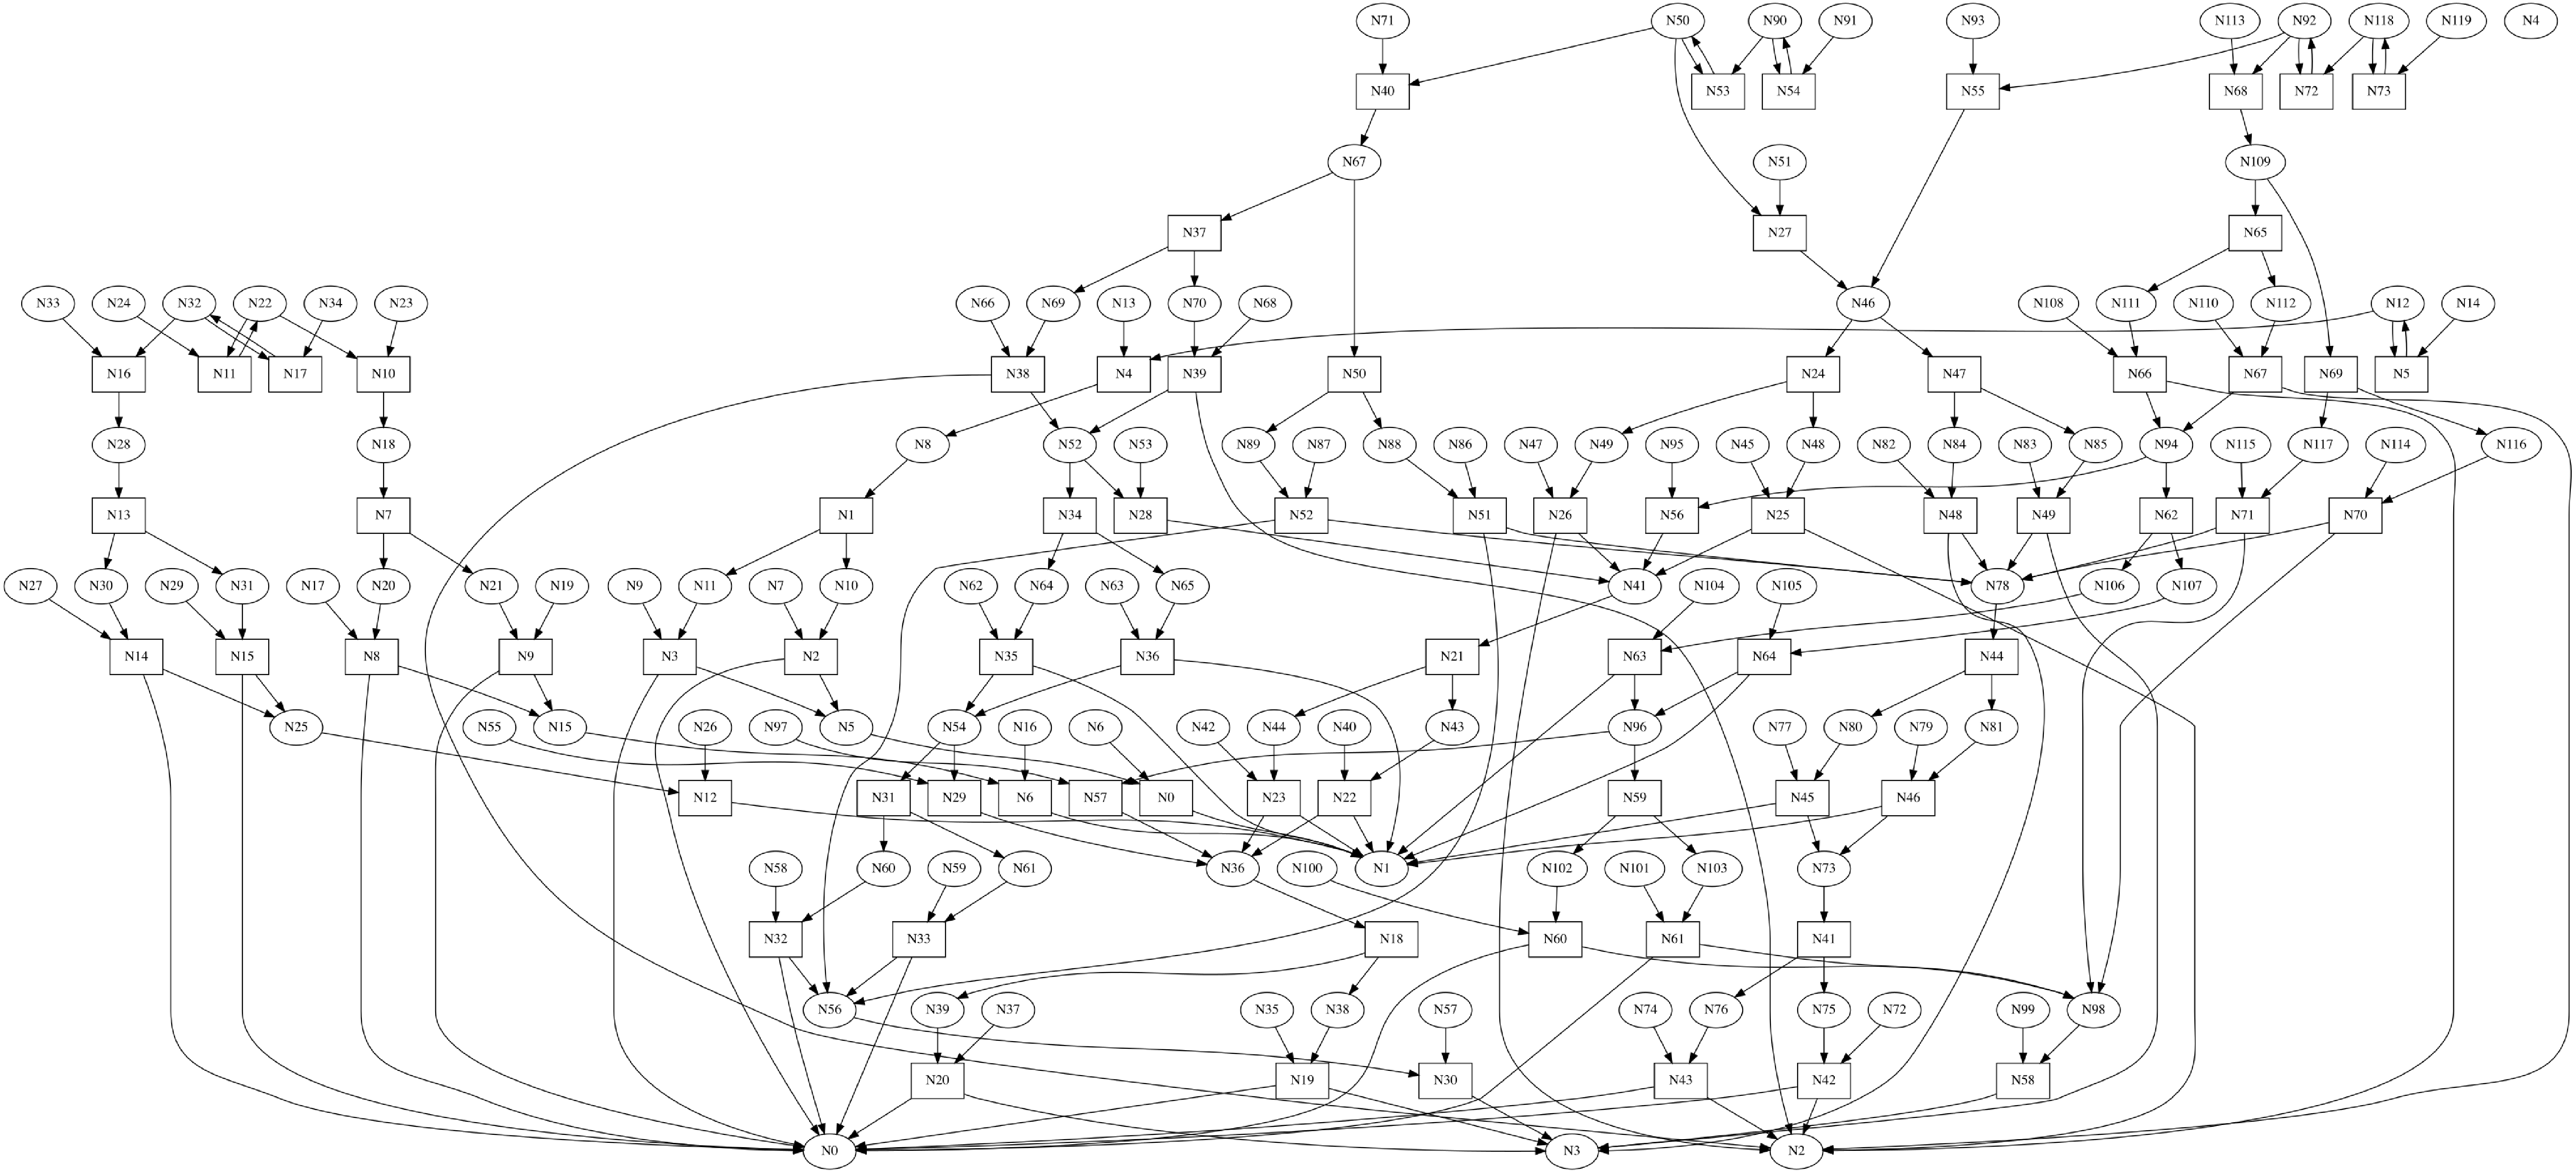
\includegraphics[width=\textwidth]{../imgs/ssb_graph.pdf}
\end{frame}



%%% Local Variables:
%%% mode: latex
%%% TeX-master: "presentation"
%%% End:


\chapter{Physical planning}
\label{chapter:physical_planning}
This chapter goes in detail about the architecture of the logical
planing of a query. Query planning is based on an A*-like search
algorithm for through the space of partial plans. We initially
describe the fundamental computational structures that facilitate this
search and their unique properties that allow us the necessary
flexibility. Then we discuss the basic backtracking algorithm and the
way the graph is traversed. We move on to discussing the garbage
collection that generates plan fragments that allow the plan to free
up space in the underlying storage. Finally we talk about the cost
model that guides the evolution of the plan.
\section{HCntT logic monad}
\label{sec:org670bd3e}
The FluiDB planner is designed in terms of a backtracking search
algorithm that searches in the space of subplans for an optimal (or
good-enough) plan. Because the algorithm involves a lot of complicated
heuristics it is important that a powerful underlying model is
deployed that matches the purely functional infrastructure in which
FluiDB is written.  We require a monad that supports both weighted
search and soft cuts. Because none of the solutions we dound in the
literature support both we we developed the \hask{HCntT} backtracking monad
that is described in this section.

\subsection{background}
\label{sec:org5cbe9b8}
Monads for backtracking in a functional context have been proposed in
various incarnateions.  The most common monad that encapsulates \hask{ListT
m a = forall b . (a -> m b -> m b) -> m b -> m b}, also dubbed the
Church encoding of lists or an application of the Cayley theorem on
list, first proposed (in an untyped format in scheme) by
\cite{haynesLogicContinuations1987}, but most authors cite
\cite{hinzeDerivingBacktrackingMonad2000a} which seems to have
redescovered an application of the concpetsin 2000, and also
\cite{kiselyovBacktrackingInterleavingTerminating} who focused on a
notion of fairness in backtracking. As shown in
\cite{kidneyAlgebrasWeightedSearch2021} this representation has
\(O(n^2)\) BFS complexity.

The other common representation of a list transformer, is the more
straightforward

\begin{haskellcode}
newtype ListT m a = ListT (Maybe (a,ListT m a))
\end{haskellcode}

Which mirrors precisely the idea behid MonadLogic from
\cite{kiselyovBacktrackingInterleavingTerminating}. As demonstrated in
listing \ref{org74ea06b} the MonadLogic able to cons(\hask{reflect}) and
uncons(\hask{msplut}).

\begin{code}
\begin{haskellcode}
class MonadPlus m => MonadLogic m where
  msplit :: m a -> m (Maybe (a,m a))
  -- ... other methods are defined in terms of msplit

reflect :: Maybe (a,m a) -> m a
reflect Nothing = mzero
reflect Just (a,as) = pure a <|> as

-- msplit >=> reflect == return
\end{haskellcode}
\caption{\label{org74ea06b}The logic monad typeclass}
\end{code}

In \cite{kiselyovBacktrackingInterleavingTerminating}, on top of this
framework they build an interleave and a monadic bind operator that
works with it to make computation be slightly more "fair".
Interleaving is fair between two computations, when more than two are
involved, half the time goes to the first computation, out of the half
that is left, half (\(1/4\) of the total) goes to the second, out of the
\(1/4\) left, half (\(1/8\)) goes to the third and so on. While this
powerseries that describes the way the way resources are allocated to
branches may seem arbitrary, in practice it may mean the difference
between terminating and non-terminating computations. For example the
code in listing \ref{org4f519db} can be translated to something like the
code in listing \ref{orgf4b45fd} which does terminates due to the fact that
while it does not give the same change to all the branches it does not
completely starve any of them.

\begin{code}
\begin{haskellcode}
nonTerm :: [(Int,Int,Int)]
nonTerm = do
  (a,b,c) <- (,,) <$> genNaturals <*> genNaturals <*> genNaturals
  guard $ a + b - c == 10
  return (a,b,c)
\end{haskellcode}
\caption{\label{org4f519db}Using a simple list to drive non-determinism is implicitly equivalent to a DFS algorithm which in many useful cases does not terminate.}
\end{code}

\begin{code}
\begin{haskellcode}
interleaveTest :: [(Int,Int,Int)]
interleaveTest = runLogic @[] $ do
  (a,b,c) <- genNaturals >*< genNaturals >*< genNaturals
  guard $ a + b - c == 10
  return (a,b,c)
\end{haskellcode}
\caption{\label{orgf4b45fd}Interleaving (in this example \hask{>*<}) is not \emph{actually} fair in the sense that it does not give all the processes}
\end{code}

So can we do better than terminating? Sometimes we can with weighted
search. Weighted search refers to the backtracking search where we
apply weights, or priority, to the branches. Branches with higher
priority are scheduled before branches with lower priority. A sketch
of the API is demonstrated in listing \ref{org77c790c}. The
backtracking monad implements the \hask{halt} operation (called \hask{tell} in
\cite{kidneyAlgebrasWeightedSearch2021}, presumably to echo the
\hask{MonadWriter} interface) which accepts a value indicating the priority
of the current branch and yields control to the scheduler. The
scheduler then passes control to the highest priority branch. The
value passed to \hask{halt} must implement a monoid such that the priority
of a branch is the concatenation of all values passed to halt up to
that point.
\begin{code}
\begin{haskellcode}
-- Todo
\end{haskellcode}
\caption{\label{org77c790c}Prioritise branches that we want to be executed first.}
\end{code}

With that in mind, for the FluiDB planner we require that our logic
framework supports the following features:

\textbf{Weighted search:} Not all plans that match our criteria, i.e. that
solve the query within the space are equally admissible. We need to
find as good plans as possible and we do not want the planner to spend
time looking into plans that are unlikely to be efficient. For that
reason neither breadth-first nor depth-first traversals are ideal for
our purpose. We need a robust way to search in a weighted manner.

\textbf{Soft-cut/either:} As we will see in more detail in the next section,
the planner is initially optimistic about being able to materialize a
node until it hits the budget limit. If the budget turns out to be
large enough FluiDB should completely disregard the the branch with
the node should be completely forgotten about. The reason is that the
later a GC happens the more options it will have and therefore the
better job it will do. To achieve that we implement an operator we dub
\hask{<//>} (pronounced \emph{eitherl}) which is similar to prolog's soft-cut.

\textbf{Once:} In the context of non-weighted search it is fairly
straightforward to demand that a subcomputation yields no more than
one value (prolog's \hask{once}). Simply run the entire computation
in-place requesting one result and if it doesn't fail return that
result. This approach can still work with weighted but we would like
the \hask{halt} calls inside the computation to have global effect for the
scheduler. In other words we want the scheduler to be able to
interleave this branch with other branches while preserving the
semantics of \textbf{once}.

None of the work we could find easily implements all the above
features simuntaneous for the FluiDB planner so we implement yet
another backtracking monad transformer, \hask{HCntT}.


\subsection{The HCntT monad}
\label{sec:org43bf21e}
The \hask{HCntT} monad combines the powers of delimited continuations and
much like \cite{kidneyAlgebrasWeightedSearch2021} it rsearches the
result in layers (see listing \ref{org7491a12}).

\begin{code}
\begin{haskellcode}
type HCntT h r m = ContT (HRes h m r)
  (ReaderT (HeapKey v)
   (StateT (CompState h r m) m))

newtype HRes h m r = HRes (Tup2 (h (Brnch h r m)),[r])
type Brnch h r m = ReaderT (HeapKey v)
  (StateT (CompState h r m) m) (HRes h m r)
\end{haskellcode}
\caption{\label{org7491a12}}
\end{code}

Here we use the continuation monad to capture the rest of the
compuation and be able to access the final result from the scope of
each operator. The result is represented as \hask{HRes} which is an
intermediate layer of the continuation. Returning empty results should
be passing. It contains a heap of halted branches and a list of
concrete evaluated valies. The heap type is parametric to allow
flexibility with respect to how to best handle the particular key
types (see listing \ref{orgf965607}). The heap is required to be stable,
i.e. items with the same key are returned in the order they were
inserted. The HeapKey \hask{mempty} must be less than (higher priority) all
other \hask{HeapKey} s.

\begin{code}
\begin{haskellcode}
class (forall v . Monoid (h v),Functor h,Monoid (HeapKey h),Ord (HeapKey h))
  => IsHeap h where
  type HeapKey h :: *

  popHeap :: h v -> Maybe ((HeapKey h,v),h v)
  singletonHeap :: HeapKey h -> v -> h v
  maxKeyHeap :: h v -> Maybe (HeapKey h)
\end{haskellcode}
\caption{\label{orgf965607}We parameterize over heaps to allow the user to decide an efficient priority queue for the branches.}
\end{code}

A halted computation branch, denoted as \hask{Brnch} is simply a
computation that evalautes to HRes. The computation must be able to
interact with CompState as required by the infrastructure supporting
\hask{<//>}.

The \hask{HCntT} on its own is not a very useful object, it needs to be
\emph{dissolved} so the values can be used. Disolution (listing
\ref{org2a763c9}) is the process of turning an HCntT value to a \hask{ListT}
value. The \hask{ListT} will lazily produce just as many results as are
required, and of course just as many effects as required, and not
more. This indicates that the process of building comptuatins is
composable but not incremental. The price of the \hask{<//>} combinator
that we described is that, unlike in other non-continuation based
monad, once we start drawing results from the computation we can not
apply further constraints on the resulting objects. Contrast that with
the case of \hask{ListT} where we can draw the first couple of results and
then use the rest in a different computation.

\begin{code}
\begin{haskellcode}
dissolve :: (IsHeap h,Monad m) => HCntT h r m r -> ListT m r
\end{haskellcode}
\caption{\label{org2a763c9}Disolution is the process of turning an \hask{HCntT} computation into a \hask{ListT}.}
\end{code}

The way disolution works then (listing \ref{orgd9e01bb}) is to first
commit to the computation constructed by applying the continuation and
obtaining an \hask{HRes}. If \hask{HRes} provides concrete results they are
yielded one by one into \hask{ListT}. Then, if the heap is not empty, the
highest priority branch is popped and scheduled to run until it yields
a new \hask{HRes}. The concrete results are yielded into \hask{ListT} and the
new heap is combined with the old one. Scheduling a branch entails
running the reader layer of the monad transformer using its pervious
value. As we will see, halting the branch will update that value
incrementally.

We use \hask{Tup2} (a functor that is simply \hask{data Tup2 = Tup2 a a}) in the
type of \hask{HRes} to allow us to be flexible on whether we use BFS or DFS
search among the same-priority branches. As mentioned when describing
the heap, a valid heap for \hask{HCntT} must be stable. While this is a
weighted search, it remains a question of how the options that have
the same priority should be ordered. If we had just one heap,
appending the newly produced heaps to the left would make for a depth
first traversal of the same-priority search space while appending on
the right would result in a breath first traversal. We want the
operators to have the flexibility to decide on which side each branch
should be appended and for that reson the \hask{HRes} actually contains two
heaps: one appended to the left (DFS), and one to the right
(BFS). This is of particular importance to the correct implementtion
of \hask{<//>} as we will see shortly.

\begin{code}
\begin{pycode}
def dissolve(branches):
    while len(branches) > 0:
        priority,best_branch = branches.pop()
        (sub_branches_left,sub_branches_right),results = best_branch.run()
        branches = sub_branches_left + brances + sub_branches_right
        for r in results:
            yield r
\end{pycode}
\caption{\label{orgd9e01bb}The dissolution algorithm in pseudo-python}
\end{code}


In the following we will briefly describe the implementations of
various combinators of \hask{HCntT}.

\subsubsection{HCntT Alternative/MonadPlus}
\label{sec:orgdfb6e7c}
The most fundamental combinator for any backtracking monad is the one
splitting branches, the implementation of \hask{Alternative} or,
equvalently in our case, \hask{MonadPlus}. The implementation for \hask{HCntT}
is fairly straightforward (listing \ref{org5991d89} ) is fairly
straightforward: for \hask{empty} or \hask{mzero}, which indicates failure of a
branch, simply disregards the continuation and returns an empty
\hask{HRes}. The \hask{mplus} or \hask{<|>} simply returns an \hask{HRes} with only the
two alternative branches having maximum priority (i.e. \hask{mempty ::
HeapKey h}) and bounded to the current continumation. Both those
branches are pushed from the right so that they are scheduled before
other same-priority branches.

\begin{code}
\begin{haskellcode}
instance (IsHeap h,Monad m) => Alternative (HCntT h r m) where
  ContT m <|> ContT m' = ContT $ \f -> return
    $ HRes (Tup2 (h (m f) <> h (m' f)) mempty,[])
    where
      h = singletonHeap mempty
  empty = ContT $ const $ return emptyHRes
\end{haskellcode}
\caption{\label{org5991d89}The implementation for \hask{Alternative} is the same as the implementation for \hask{MonadPlus}.}
\end{code}


\subsubsection{HCntT halt}
\label{sec:org16bc12a}
We mentioned the \hask{halt} \hask{HCntT} process. Because we want to be able to
transform the \hask{HCntT} monad we define the class of \hask{MonadHalt} that
can support this operation. Most common monad transformers of \hask{HCntT}
can trivially support halt. The implementation of \hask{halt} for \hask{HCntT}
itself is demonstrated in listing \ref{orge4516d6}. The provided
priority is offset by the previous priority of the branch.

\begin{code}
\begin{haskellcode}
class Monad m => MonadHalt  m where
  type HaltKey m :: *
  halt :: HaltKey m -> m ()

instance (Monad m,IsHeap h) => MonadHalt (HCntT h r m) where
  type HaltKey (HCntT h r m) = HeapKey h
  halt v = ContT $ \nxt -> do
    v' <- asks (v <>)
    return $ HRes (Tup2 (singletonHeap v $ nxt ()) mempty,[])
\end{haskellcode}
\caption{\label{orge4516d6}The halt process yields updates the priority of the branch and yields execution to the scheduler.}
\end{code}


\subsubsection{Soft-cut/eitherl}
\label{sec:orgba03e8f}
The \hask{<//>} (pronounced eitherl), \hask{left <//> right} runs the left hand
side operand (primary) and if no values are produced in the \emph{entire}
computation based on that, only then does it try to evaluate the right
hand side (fallback). \hask{HCntT} does not guarante that the right hand
side will be scheduled immediately after it realizes that there are no
solutions, but it does guarantee that it will be scheduled before it
moves on to a new priority. In other words it is only guarantted that
the priority of the fallback branch will tie the last failing branch
of the left hand side in terms of priority, but if there are other
branches that tie, there is no guarantee of how those will be
scheduled.

There are two challenges that our particular feature set imposes to
implementing this:

\begin{itemize}
\item We want \hask{<//>} to operate on the entire operation, unlike
\cite{kiselyovBacktrackingInterleavingTerminating} that makes the
decision o whether to run the fallback solely based on whther the
left hand side returns a value.
\item In the context of a weightedx search control needs to be able to
escape a branch that passes through the left hand side operand
before it is exhausted. Therefore we can not simply dissolve the
left hand side and reconstruct it. But then how would the operator
know when the branches are exhausted?
\end{itemize}

We solve these problems with the use of a special kind of branch we
call a \emph{marker}, and a global state. Since branches are arbitrary
processes we equip them with access to global state (local to the
computation), a lookup table (\hask{CompState}) full of fallback
branches. The main ideas is that a fallback branch corresponds to an
entry int the lookup table. This entry is modified accordingly by the
children of the right hand side. At the time of the cut we push a
marker into the heap with priority lower than the child branches so
that when it is scheduled it will perform some checks based on the
lookup table entry and schedule the fallback function if all the
children branches have finished whithout a result.

We will see in a bit how the contents of the lookup table are updated
and how new, lower priority markers are pushed in the heap. For now
consider that each marker may be superseded by a lower priority marker
rendering it a invalid. At any time there is exactly one valid marker
per active fallback and it is denoted as such by the fallback entry in
the lookup table. The rest of makers are invalid and should be
equivalent to noops.

More precisely about the internals of the marker processes, each one
refers to a location in the lookup table via its closure. Also each
marker is uniquely identifiable so each valid entry in the lookup
table references one marker. Specifically the lowest priority one that
corresponds to it. When the marker is scheduled it looks up the
fallback branch entry in the table and checks if the entry also refers
to that marker. There are 3 possible scenaria that may play out at
this point:

\begin{itemize}
\item The fallback entry in the table has been invalidated by a branch
that yielded a result. In this case the marker is invalid and just
returns.
\item The fallback entry is valid but does not correspond to the scheduled
marker. This means due to the left hand side branch spawning low
priority sub-branches, another marker has been inserted to
(possibly) trigger the fallback at some time in the future. The
current marker is invalid
\item The fallback location is valid and corresponds to the scheduled
marker. This means that it is time fallback process needs to be run
and removed from the table.
\end{itemize}

But what is the lifecycle of the fallback entries? When an exprssion
\hask{A <//> B} appears we create a new fallback entry in the lookup table
containing \hask{B} and recursively "infect" all spawned sub-branches of
\hask{A} to perform the following actions immediately after they generate
new branches and results:

\begin{itemize}
\item If there is at least one valid result invalidate the fallback in the
lookup table and stop infecting child branches with the currently
described hook.
\item If the fallback is invalid it means there have already been valid
results that rendered the fallback obsolete. Stop infecting
sub-branches.
\item If none of above happened check the priority of the last marker
corresponding to the fallback (registerd in the lookup table
entry). If it is strictly lower than the lowest priority
subbranch do nothing because there is a well placed marker to
handle it. Otherwise create a new marker of the same priority as
the lowest priority subbranch and put it in the right-append
heap. This way we know it will be scheduled AFTER the last branch
relating to the fallback.
\end{itemize}


It is demonstrated in figure \ref{fig:org90c1788}


\begin{figure}[p]
\centering
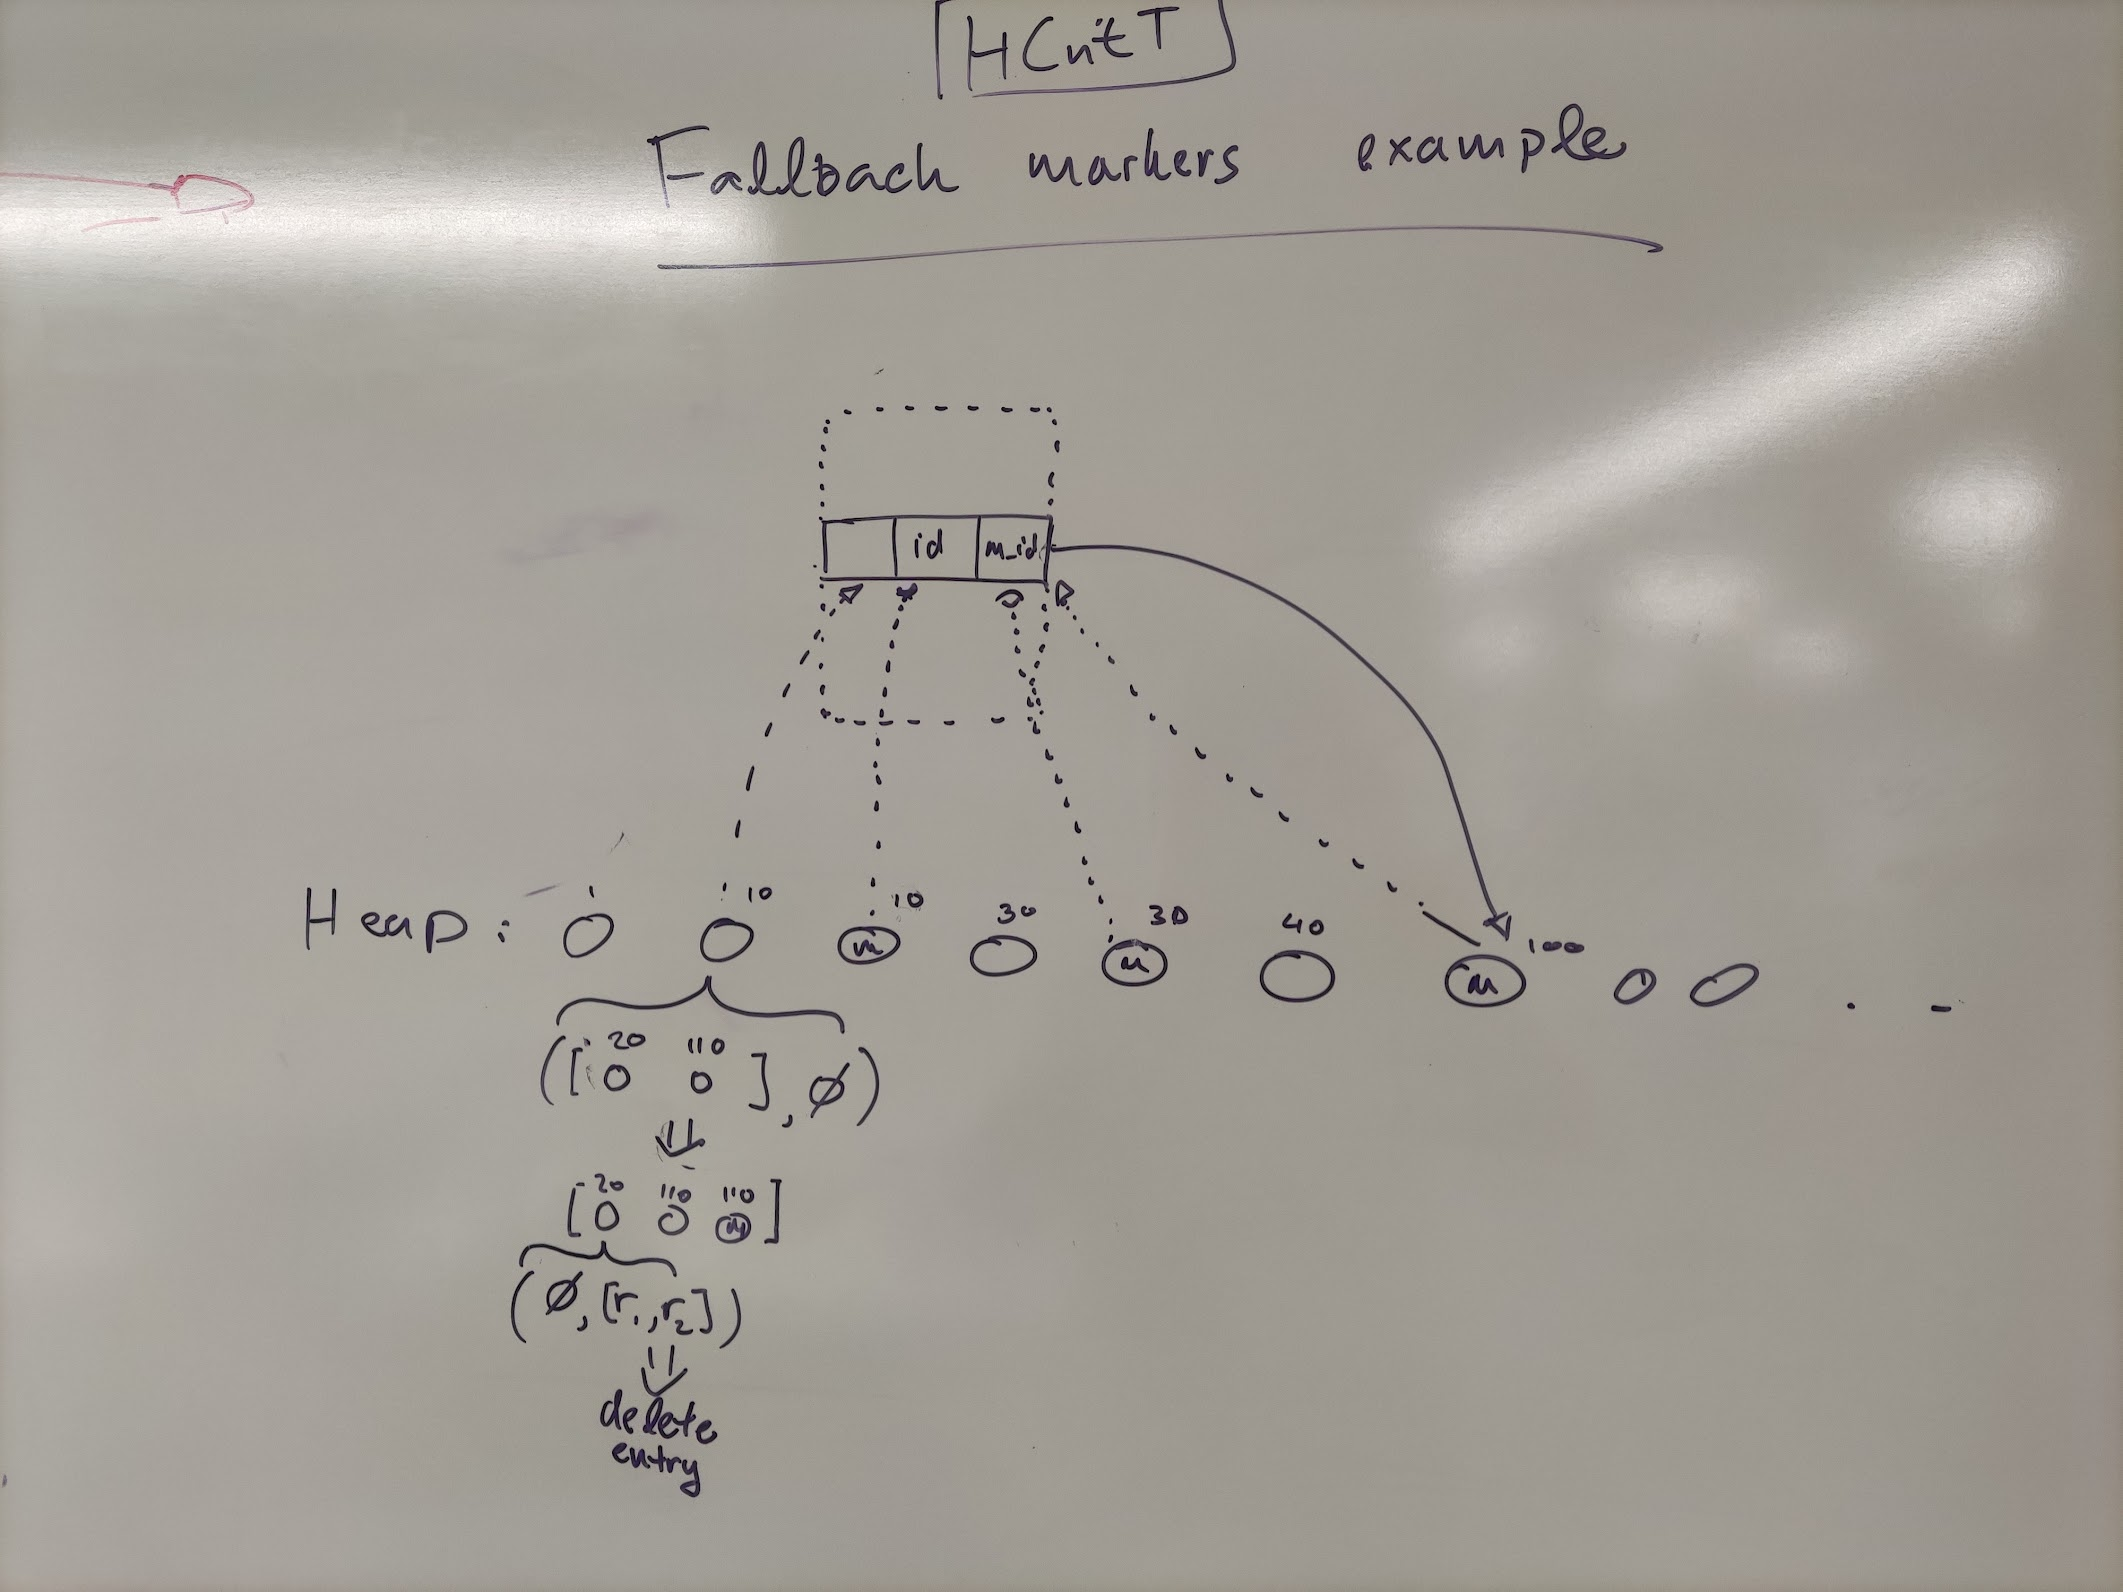
\includegraphics[width=.9\linewidth]{./imgs/2021-10-28_13-20-45_screenshot.png}
\caption{\label{fig:org90c1788}Marker "branches" are injected in the
  heap of prioritized branches to possibly trigger the fallback
  branch. Each marker gives the scheduler the opportunity to run a
  particular fallback branch. The entry of the fallback branch entry
  references the last marker so that only that one actually trigger
  the fallback branch. A child branch that succeeds removres the
  fallback entry so the final marker also fails to tigger the
  fallback.}
\end{figure}



There are some optimizations that can be implemented to avoid too many
lookups in the fallback table in the case of deep eitherl nesting that
take advantage of the fact that new markers for outer fallbacks may
only be created when new markers for inner fallbacks are
created. However, for FluiDB we did not find \hask{CntT} to be too bad of a
performance bottleneck so we leave it for future work.


\subsubsection{Once}
\label{sec:orgf87066e}
The \hask{once} operator runs the argument computation and stops once it
returns the first result. FluiDB uses \hask{once} to run the garbage
collector without exploding the search space. Generally the different
combinations of nodes that can be deleted is huge. We prune that by
space by settling for the first result the solver can find.

The way \hask{Once} is built on top of a concept we call a \emph{nested
scheduler}. It takse a computation (the \emph{nested computation}) and
needs to know what to do in case of a success and in case of complete
failure (no more branches to run). The nested scheduler is a process
that \emph{always} returns a single case subbranch. This subbranch has the
priority of the highest priority subbranch of the nested computation
and when scheduled it internally schedules the next branch of the
nested process. When the process yields results or fails completely
the corresponding hook is run. \hask{once} implements these hooks as
"return the result and stop" and as "propagate the failure"
respecively. Since the implementation of \hask{once} is fairly small it is
provided along with the types in listing \ref{org246cc16}.

\begin{code}
\begin{haskellcode}
nested
  :: forall h m r a .
  (Monad m,IsHeap h)
  => (Tup2 (h (Brnch h r m)) -> r -> [r] -> HRes h m r)
  -> HRes h m r
  -> HCntT h r m a
  -> HCntT h r m a
nested success fail c = ...

once :: forall h m r a . (Monad m,IsHeap h) => HCntT h r m a -> HCntT h r m a
once = nested (\_h r _rs -> HRes (Tup2 mempty mempty,[r])) emptyHRes
\end{haskellcode}
\caption{\label{org246cc16}The nested scheduler runs a subprocess within a single branch. Once is built on top of that to make sure the process stops once a result is returned.}
\end{code}


It is worth noting that nested schedulers are also applicable of
implementing \hask{<//>}. In the marker-based implementation we are
performing \(N\) lookups on the fields table, \(N\) being the nesting
of \hask{<//>} operators. Implementing it using nested schedulers, on the
other hand, means we are doing \(N\) pop/push pairs, one for each
nested heap. For FluiDB we use a slighltly too general notion of a
heap so we opt for the former.
\section{The planner}
\label{sec:org3e22e01}

\subsection{Traversing the graph}
\label{sec:orgad5ab39}
The planner is the subsystem of FluiDB that given the state of the
QDAG and a target node to be materialized produces a logical plan that
will materialize the query.  Our notion of a logical plan is slightly
more specific them what is commonly considered a logical plan,
i.e. the RA representation of the query. In our case it is a sequence
of \emph{transitions} that are to be transpiled to C++ by the code
generator. There are three kinds of transitionse:

\begin{itemize}
\item t-node trigger that assumes the input n-nodes are materialized and
produces a subset of the output nodes.
\item t-node reverse trigger that assumes that the output nodes are materialized
\item n-node deletion
\end{itemize}

The planner operates by backtracking using \hask{CntT} monad. Each branch
mainains some branch-internal effects that are reified as monad
transformers on top of the \hask{CntT} defining the \hask{PlanT} monad
transformer (listing \ref{org0ac3c80}).

\begin{code}
\begin{haskellcode}
type PlanT t n m =
  StateT
    (GCState t n)
    (ReaderT (GCConfig t n)
     (ExceptT (PlanningError t n)
      (HCntT PlanHeap () m)))
\end{haskellcode}
\caption{\label{org0ac3c80}The monad that defines all the useful effects used by the planner. \hask{GCConf t n} is an immutable, from the persepctive of the planner, configuration that includes the QDAG, the node sizes, etc. \hask{GCState t n} is state that is mutated and private to each branch of the planner like the materialized status of the nodes, the set of transitions registered so far and various caches. The \hask{PlanningError t n} is a planner specific type of error. The entirety of the result of planning is accumumated in \hask{GCState} so the result of backtracking is just unit (\hask{()}).}
\end{code}

It is important to clarify the way we use the term "materialized node"
(\hask{Mat} as opposed to "not materialized" -- \hask{NoMat}) from the planner's
perspective. A mapping of node states is passed to the planner at the
beginning of the planning process. This mapping indicates which nodes
are initially materialized. Then as transitions get registered update
the mapping is updated to reflect the effect that the plan so far
would have on the materialized relation set in storage. Since the
planner operates via backtracking (using the \hask{CntT} monad described),
each branch maintains its own mapping of node states and therefore
considers a different set of materialized nodes.

We maintain the partial plan (sequence of transitions) as part of the
state of each of the planners branches. Registering a transition means
that a transition is added to the partial plan.

The main loop of the planer is a recursive process of asseerting that
nodes are materialized. If the node is already materialized the
assertion succeeds, if not the planner attempts to trigger, or reverse
trigger, a neighbouring t-node that would lead to the node being
materialized, asserting first that the input nodes of that transition
are materialized. In practice, due to intermediate n-nodes being
auxiliary and not corresponding to real nodes, we know that t-nodes
are organized in sequences that need to be triggered entirely or not
at all. For example (figure \ref{fig:org8fe4b6e}) the intermediate
\(\lsemi\) nodes are not actually materialized as part of the join
operator. Equipped with this knowledge we organize the t-nodes into
\hask{MetaOps} (listing \ref{org682fa71}) that can atomically be triggered or
reverse triggered. \hask{MetaOps} also abstract the distinction between
triggering and reverse triggering as they expose a set of input, a set
of output nodes and a process that registers the correct transitions
once the \hask{MetaOp} is triggered. The process of asserting asserting an
n-node being materialized then becaomes the process of
non-deterministically selecting a \hask{MetaOp} with the node in question
in the output set. Before actually splicing the \hask{MetaOp} compiutation
we assert that the input set is materialized.


\begin{figure}[p]
\centering
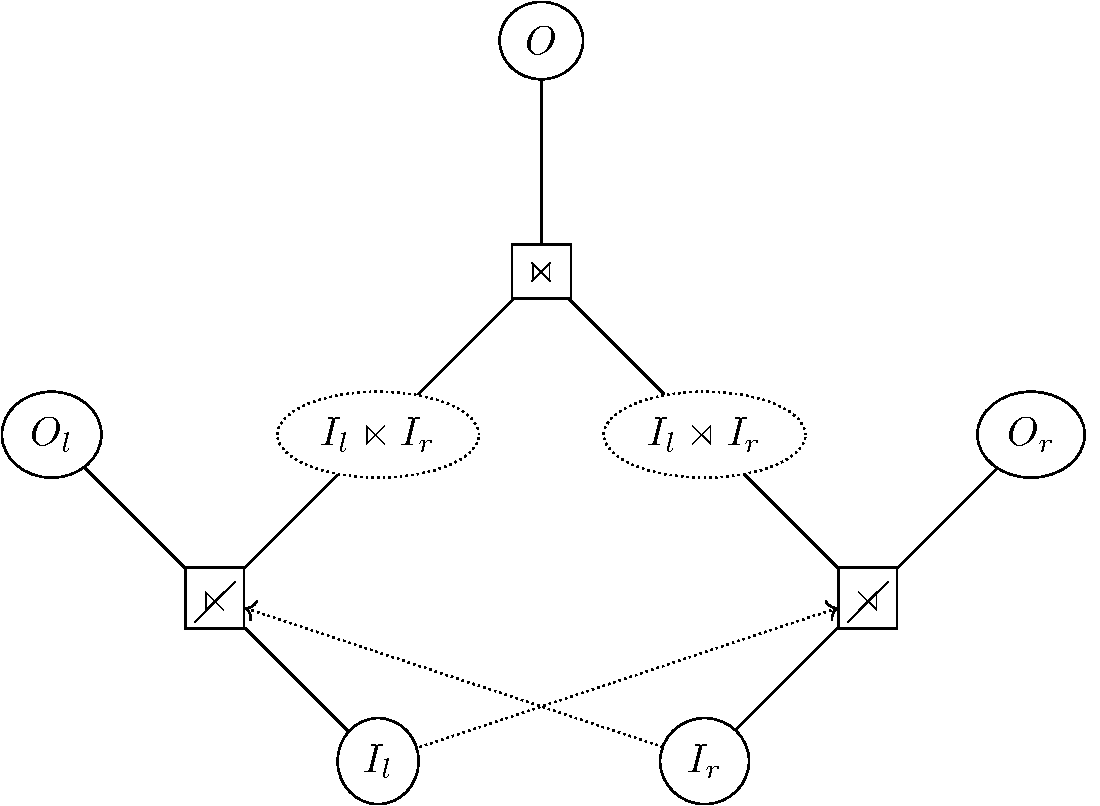
\includegraphics[width=.9\linewidth]{./imgs/example_metaop.pdf}
\caption{\label{fig:org8fe4b6e}starting at node \(O\), the output of a join operation, we can derive three MetaOps that can materialize it.  \(MetaOp\{in: \langle I_l, I_r \rangle, out: \langle O \rangle \}\), \(MetaOp\{in: \langle I_l, I_r \rangle, out: \langle O_l, O \rangle \}\), \(MetaOp\{in: \langle I_l, I_r \rangle, out: \langle O, O_r \rangle \}\), \(MetaOp\{in: \langle I_1, I_2 \rangle, out: \langle O_l, O, O_r \rangle \}\). Because trying all combinations of outputs explodes the seach space we always go for the largest and then let the garbage collector deal with the possible reprecussions. On the other hand to materialize \(I_l\) there is only one \hask{MetaOp} that relates to this cluster \(MetaOp\{in:\langle O, O_l \rangle, out: \langle I_l \rangle, interm: \langle I_l \lsemi I_r \rangle \}\)}
\end{figure}

\begin{code}
\begin{haskellcode}
data MetaOp t n = MetaOp {
  metaOpIn     :: NodeSet n,
  metaOpOut    :: NodeSet n,
  metaOpInterm :: NodeSet n,
  metaOpPlan   :: forall m' . Monad m' => PlanT t n m' [Transition t n]
  }
\end{haskellcode}
\caption{\label{org682fa71}A \hask{MetaOp} refers to input, output, and intermediate nodes that are involved in the set of operations it abstracts. Furthermore it contains a computation that registers and returns the transitions involved in the \hask{MetaOp}.}
\end{code}


Two questions should arise from the above description: a) how does the
planner avoid cycles where it recursively tries to materialize the
parents and then the children? and b) how does it know not to
materialize a node twice? Both those problems are addressed by
refining the possible states of the n-nodes (listing
\ref{orge1e857d}). Rather than being just \hask{Mat} or \hask{NoMat}. We also
disambiguate between \hask{Initial} and \hask{Concrete} nodes. Nodes in the
\hask{Initial} state are allowed to change their materialization status. In
contrast \hask{Concrete} nodes have their state fixed with very few
exceptions. Then, when a node is asserted to be materialized its
status is first checked and followin scenaria are possible:

\begin{itemize}
\item the node's status found to be \hask{Concrete} and \hask{NoMat} and the branch
immediately fails as it is not allowed to be set to materialized.
\item if it is \hask{Concrete} and \hask{Mat} the assertion simply succeeds
\item If it is \hask{Initial} and \hask{Mat} it is turned into \hask{Concrete} and \hask{Mat}
and the assertion succeeds.
\item if the node's status is \hask{Initial} and also \hask{NoMat}, two things need
to happen: first the node is set \hask{Concrete} and \hask{NoMat} in order to
avoid cycles, and the aforementioned process of finding a \hask{MetaOp}
is carried out recusively in order to materialize the node.
\end{itemize}

\begin{code}
\begin{haskellcode}
data IsMat = Mat | NoMat
data NodeState =
  -- Concretified states are allowed to change only within the same
  -- lexical scope.
  Concrete IsMat
  -- Initial states are subject to change when encountered as a
  -- neighbour or by the GC.
  | Initial IsMat
\end{haskellcode}
\caption{\label{orge1e857d}The different states that a node is allowed to be in.}
\end{code}


Once an n-node's is materialized and we start materializing its
siblings, it is important that the garbage collector (which we will be
discussing in the next section) does not delete said n-node.  To avoid
this problem, items materialized are set to \hask{Concrete Mat} until all
their siblings, that are inputs to the same \hask{MetaOp}, are
materialized. Once the \hask{MetaOp} is triggered and its output nodes are
set to the \hask{Concrete Mat} state the input nodes are set to \hask{Initial
Mat} as it is now safe for the garbage collector to remove them.

It is worth noting here the importance of every node in the depset
being completeley materialized before the process of materializing the
next one comences. The reason is that at any time a single trail of
parent nodes is marked as \hask{Concrete} and \hask{NoMat}, otherwise we can't
be sure whether a \hask{Concrete NoMat} node that renders a \hask{MetaOp}
non-triggerable is actually in the process of becoming materialized,
meaning that when that process succeeds the \hask{MataOp} under
consideration will be triggerable.
\subsection{Garbage collection}
\label{sec:org1089d97}
One of the fundamental design decisions of FluiDB is that it is
commited to materializing all intermediate nodes and keeping them
around for as long as possible. In one hand the plan selected is
crafted so that the intermediate results are maximally useful for the
overall workload, on the other, when the available storage runs out,
the garbage collector mechanism selects the least useful nodes to be
deleted, creating free required for solving the query. In this section
we focus on the latter.

The garbage collector is triggered right before a \hask{MetaOp} is to be
triggered. It infers the space required for materializing the output
nodes and the space available to decide how much space is
required. Then it selects a subset of materialized nodes to delete in
order to make room for the new results. The selection process has two
hard constraints:

\begin{itemize}
\item The nodes being deleted must be \emph{deletable}, i.e. the node's state
is \hask{Initial} and if the node is deleted it can be reconstructed from
the remaining materialized nodes.
\item The nodes being deleted must not be required for the continuation of
the current plan. We call these nodes \emph{protected}. For example, say
we are planning for the query \(A \Join B\) and we have materialized
\(A\) already but while materializing \(B\) the GC is
triggered. \(A\) should not be in the repertoire of nodes the GC can
delete under any circumstances.
\end{itemize}

Selecting a subset of nodes is not an easy problem so we follow a
simple heuristic and leave a proper solution for future work.

Large nodes are costly to create and therefore the larger the node,
the less inclined the planner is to create it, and the more useful it
is likely to be. With that in mind the heuristic we follow is for the
garbage collector to prioritise deleting small nodes over deleting
larger ones. The first order of business for the GC the is to find the
set of deletable nodes and sort them by size. It tries to delete them
one by one starting from the smaller ones and working its way up to
the larger ones. Every time a node is deleted it is possible that
other nodes that were previously established to be deletable lose that
property. For example if all nodes \(A\), \(\sigma_p A\), and
\(\sigma_{\neg p} A\) are \hask{Initial} and materialized, each one of them
can be materialized from the others and therefore all of them are
marked as deletable. If the GC deletes \(\sigma_p A\) first the other
two are no longer materializable as they depended on \(A\) to be
materializable.

Nodes that are established as non-deletable in this way are switched
from \hask{Initial} to \hask{Concrete} to avoid re-calculating their
materializability.

If after this process not enouch space was created, the GC resorts to
starting a new \emph{planner epoch}. When a new planner epoch begins all
the nodes states and transitions that were recorded since the last
planner epoch started are stashed into the epoch stack. The epoch
stack resides in the branch-local state (\hask{GCState}) and contains a map
of nodes to their states at the end of the epoch and a sequence of
transitions. When a new epoch is pushed into the stack a new mapping
of states is created according to the following rules:

\begin{itemize}
\item The materialization status does not change between epochs: All
materialized nodes from the previous epoch are materialized in the
new one materialized and all non-materialized nodes are still not
materialized.
\item All non-protected \hask{Concrete} nodes become \hask{Initial} nodes.
\end{itemize}

The sequence of transitions for the new epoch is empty. The reason we
keep separate lists of transitions is, as we will see in more detail
in the code generation chapter, that the subset of output nodes that a
physical operation generates is established at the time of physical
planning based on the materialized nodes according to the epoch
corresponding to the transition.

An epoch contains all the important information about the state of the
planner. For this reason when an epoch is inserted in the stack it is
checked for equality against the other epochs in the stack. If two
equivalent epochs are inserted in the stack the branch fails
permanently as it means that there is a cycle.

This enables another optimization, the \emph{free-to-delete} nodes. As
mentioned previously the planner prioritizes the version of \hask{MetaOps}
that materializes all the outputs for example it will prioritize the
branch that followes \(MetaOp\{in=\langle A \rangle, out=\langle
\sigma_p A, \sigma_{\neg p} A \}\) over the on that follows
\(MetaOp\{in=\langle A \rangle, out=\langle \sigma_p A \}\). It is
rarely the case, however, that all the outputs are required. In the
example just mentioned then the former example, triggering the former
\hask{MetaOp} and then garbage collecting \(\sigma_{\neg p} A\) without it
being used is never desirable. For that reason we mark the node
\(\sigma_{\neg p} A\) as \emph{free-to-delete} as soon as it is created
based on the fact that it is not required. When the garbage collector
deletes free-to-delete nodes it does so without registering a deletion
transition. This way the physical planner will generate a plan where
\(\sigma_{\neg p} A\) is never created in the first place. All nodes
lose their free-to-delete status upon the creation of a new epoch.

The comprehensive algorithm for the GC is presented in listing \ref{orgce398cd}

\begin{code}
\begin{haskellcode}
gc reqSize = do
  -- Try the current epoch and if that fails retry with a new epoch.
  return () <//> newEpoch
  -- find the deletable nodes and sort them by size
  deleteables <- sortOnM getNodeSize =<< filterM isDeletable =<< getAllNodes
  -- Try deleting each node and stop deleting when amassing enough
  -- free pages.
  forM_ deletables $ \n -> do
    freePgs <- getFreePages
    when (freePgs < reqSize) $ tryDelete n <//> markAsConcrete n

tryDelete node = do
  guardM isDeletable
  isFreeToDel <- getIsFreeToDel node
  unless isFreeToDel $ register $ DelNode node
  setStatus node (Initial NoMat)

isDeletable n = do
  st <- getNodeState n
  case st of
    Initial Mat -> do
      setNodeState n (Initial NoMat)
      ret <- isMaterializable n
      setNodeState n (Initial Mat)
      return ret
    _ -> return False

markAsConcrete = do
  st <- getNodeState n
  case st of
    Initial m -> setNodeState (Concrete m)
    _ -> return ()
\end{haskellcode}
\caption{\label{orgce398cd}A sketch of the garbage collector algorithm in pseudo-haskell. The \hask{<//>} operator  is supported by the \hask{HCntT}.}
\end{code}

The garbage collector may have a final trick up their sleeve when all
else fails: neighbor materialization. When there exists a dependency
set of a non-deletable node that takes up less size that the node
itself, the transition, the GC can attempt to trigger the
corresponding \hask{MetaOp} in order to generate the dependency set and
render the node deletable. For example the \(\theta\)-join node \(A
\Join_\theta B\) is likely to take up more space than \(A\) and \(B\)
combined. This makes the search space explode and is a generally
low-yield strategy, therefore it is by default disabled.

It is hopefully clear at this point that the process of garbage
collection involves a huge search space. We sacrifice a some of our
plan repertoire by running the entire process wrapped in a \hask{once}
operator that we described in the previous section.

Finally, a word about protected nodes. Nodes are protected within the
context of a branch from the time they are established as part of the
input set of a \hask{MetaOp} we are making trigerable until the time said
\hask{MetaOp} is actually triggered during the normal planning (i.e. not
the GC). Because a node may be the input of more than one
simultaneously considered \hask{MetaOps}, protection of a node is not a
boolean value that is set when the node is encountered as \hask{MetaOp}
input and unset when the \hask{MetaOp} is triggered, but rather an natural
number variable that is incremented and decremented respectively. When
that value is zero, the node is not considered to be protected.


\subsection{Order of traversal}
\label{sec:org2851b35}
We mentioned that the \hask{MetaOps} are selected non-deterministically. In
this section we will go in depth on the FluiDB planner's strategy on
the order in which it considers its options using the \hask{CntT}
framework, making heavy use of the \hask{halt} operator to set priorities
for branches. A branch's priority is dependent on the particular
frontier at the time of a halt and is determined by four factors:

\begin{itemize}
\item The cost of the MetaOps that the branch is in the process of making
trigerable.
\item The cost of the MetaOps that have already been triggered.
\item The sum of the estimated costs of each node in the frontier.
\item A weighted sum of the \emph{stochstic cost} of historical queries based
on the current frontier.
\end{itemize}

The final two factors are values, on which we will focus in this
section, are computed often and are dependent on the set of
materialized nodes. Since the set of materialzied nodes does not
change in a completely arbitrary way from computation to computation a
naive approach to calculating those values would involve a lot of
duplicate work. For this reason we use Antisthenis which will be
expanded in a separate chapter to minimize the amount of work
required.

Let's start with the sum of estimated costs. We have a very rough way
of estimating costs. We incrementally estimate the cost of each node
of the frontier using the following formula:

\begin{align}
  c_{nomat}(n) &=
    \min\limits_{op \in \text{metaops with \(n\) output}} \left\{ cost(op) + \sum\limits_{i \in inputs(op)} c(i)  \right\} \\
  c_{mat}(n) &= 0
\end{align}

Where the cost \(c\) is \(c_{mat}\) if the cost is materialized and
\(c_{nomat}\) otherwise. In plain english the cost is recursively
estimated as cheapest combination \hask{MataOp} plus the cost of
materializing the input nodes.

This approach has several problems like the fact that nodes that are
used more than once are added more than once and that it does not take
at all into account the budget constraints. It is, however, a good
enough heuristic for prioritizing the branch.

The final factor, which takes into account the historical queries is a
bit more tricky. The planner keeps track of the last couple of nodes
materialized previously and tries to estimate how useful beneficial
following the particular branch would be in the event where a query
similar to those is requested in the future. We estimate that by
summing up a notion of cost for those queries.

A naive approach would be to just use the the same algorith as we did
for the frontier nodes. However, this approach is prone to getting
stuck behind materialized nodes. However, this approach is
prone to getting stuck behind materialized nodes. Past queries,
epsecially recent ones are likely to still be materialized and
therefore their cost is likely to be 0. Even if the GC has gotten
around to deleting them, their near dependencies are likely to block
the cost estimator go far. This makes the estimation quite bad for two
reasons:

\begin{itemize}
\item The planner is likely to have deleted any number of materialized
nodes that the cost estimation may be depending on.
\item We don't care about the cost of the particular nodes, but rather
about \emph{similar} nodes. For that reason we want to avoid depending
too heavily on a particular materialized node being there.
\end{itemize}

A realistic way of calculating the expected cost of a node in the
future, which we very informally and heuristically attempt to
approximate, would be to instead of considering the cost of
materialized nodes to be zero, to calculate the likelihood that a
materialized node will still be materialized when we encounter it
again. This is related not only to an estimation of how many
page-writes separate the moment of cost estimation and the actual plan
the cost of which is being estimated, but also all the decisions that
the garbage collector will make in that time. After FluiDB's budget is
exhausted for the first time, for every page write there a page needs
to be garbage collected. We considered a couple of options for
stochastically modelling the behavior of the GC like assuming that it
chooses random pages or random tables, but we could find none that was
useful and computationally viable.

For this reason we decided to follow a pragmatic approach to the
problem and simply assume that for every materialized node there is a
constant probability that it will not still be materialized when we
need it, scaling the cost by that factor to get the stochastic
cost. So the cost formula \(h\) for the nodes now is:

\begin{align*}
  h_{nomat}(n) &= \min\limits_{op \in \text{metaops with \(n\) output}} \left\{ h(op) + \sum\limits_{i \in inputs(op)} cost(i)  \right\} \\
  h_{mat}(n) &= \lambda \cdot h_{nomat}(n)
\end{align*}

Where \(\lambda \in (0,1)\) is the estimated probability that the the
node is still materialized when needed. As before materialized nodes
have cost \(h_mat\) and non-materialized nodes have cos \(h_{nomat}\)


\chapter{Antisthenis}
\label{chapter:antisthenis}
\begin{frame}
  \frametitle{Antisthenis}
  \framesubtitle{Dynamically scheduled incremental computation}

  Materializablility and cost inference are numerical operations:

  \begin{itemize}
  \item Input is mostly the same between runs: \textbf{incremental}.
  \item \textbf{Order of computation} highly affects the performance
    (eg absorbig elements, min).
  \item Self referrential computations may appear earlier than the
    absorbing element.
  \end{itemize}
\end{frame}


\begin{frame}{Antisthenis: Expression graphs}
  \framesubtitle{Variable name \(\mapsto\) expression, leaf variables }
  \begin{columns}
    \begin{column}{0.5\textwidth}
      \begin{align*}
        A &= a + B + C + D  \\
        B &= C \times b \\
        C & = D + c \\
        D &= 0
      \end{align*}
    \end{column}
    \begin{column}{0.5\textwidth}
      \begin{center}
        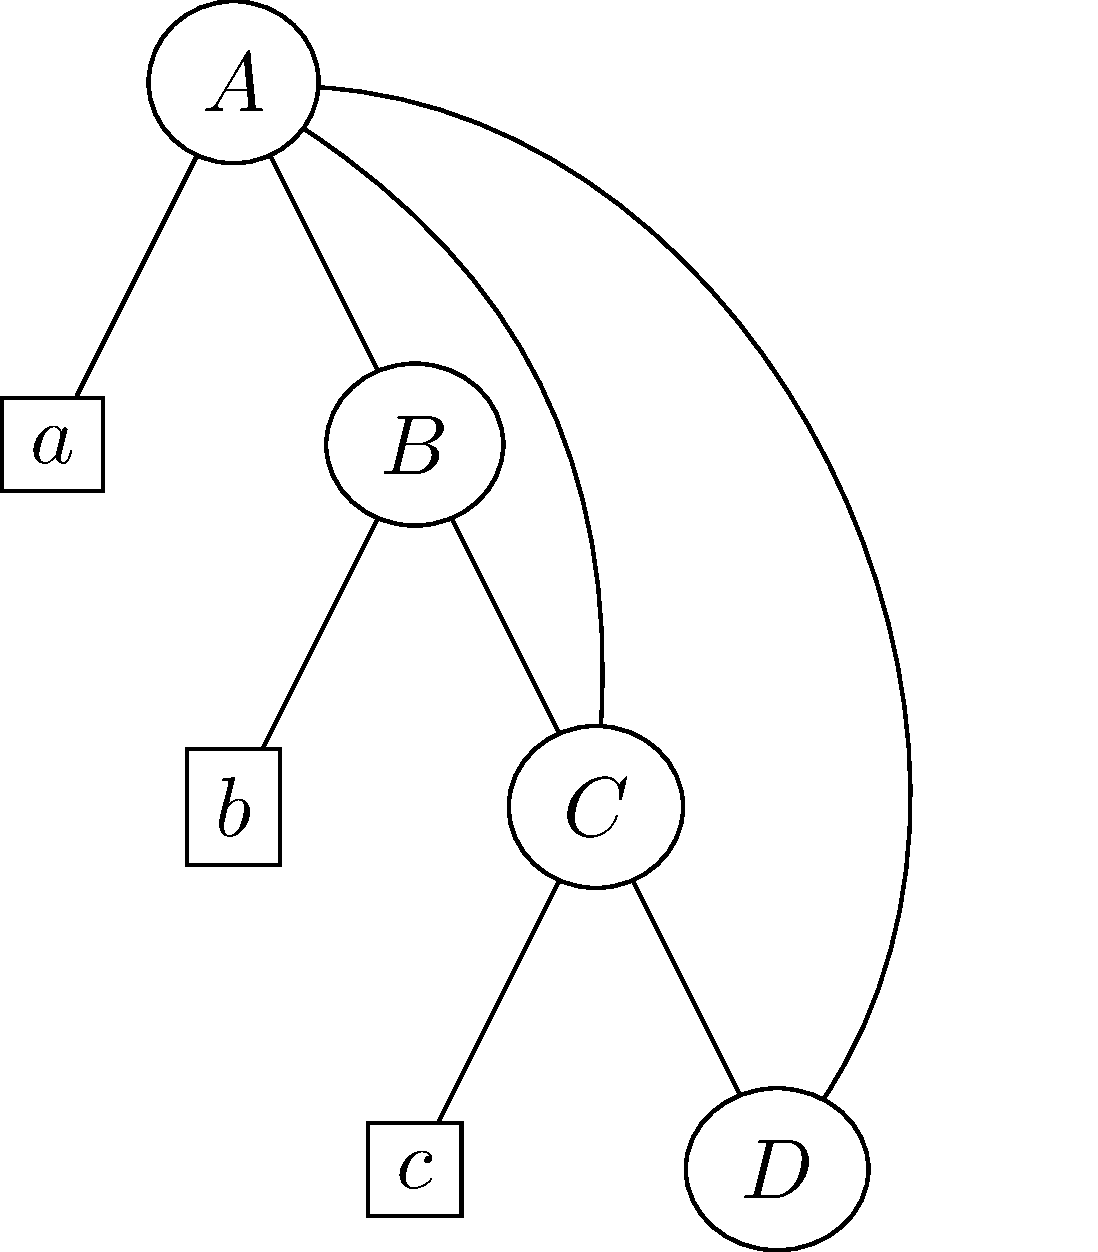
\includegraphics[height=.6\textheight]{../imgs/example_antisthenis_dag.pdf}
      \end{center}
    \end{column}
  \end{columns}
\end{frame}


\begin{frame}
  \frametitle{Antisthenis: Absorbing element}
  \begin{align*}
    A &= {\color{red}B} \times {\color{gray}C} \times D \\
    {\color{red}B} &= {\color{red}\sum_i{i}} \\
    {\color{gray}C} &= {\color{gray}10 - 10} \\
    D &= \sum_i{i}
  \end{align*}
\end{frame}


\begin{frame}{Antisthenis: Early stopping -- recursive expressions}
  {While expressions may be self-referential, we can
    sometimes still evaluate them.}
  \begin{align*}
    A &= min({\color{red}B}, C, {\color{blue}D}) \\
    {\color{red}B} &= b_1 + b_2 \cdot {\color{blue}D} \\
    C &= c_1 + {\color{gray}c_2 \cdot A} \\
    {\color{blue}D} &= d_1 + d_2 \cdot {\color{red}B} \\
  \end{align*}
  \hrule
  \begin{align*}
    b_1 &= b_2 = d_1 = d_2 = 1 \\
    c_1 &= 3 \\
    c_2 &= 0
  \end{align*}
\end{frame}

\newcommand{\wlor}{\mathop{\bigvee}\displaylimits}
\newcommand{\wland}{\mathop{\bigwedge}\displaylimits}
\begin{frame}{Kinds of operations: Materializability}
  \[
    matable(n) := \wlor_{depset \in depsets(n)}\wland_{dep \in depset} mat(dep) \lor matable(dep)
  \]
  \uncover<2>{
    \begin{itemize}
    \item Recursive -- normally we would maintain a visited set.
    \item Incremental evaluation is inhibited.
    \item Bot \(\land\) and \(\lor\) have absorbing elements.
    \end{itemize}}
\end{frame}

\begin{frame}{Kinds of operations: Estimated cost}
    \[
  \scalebox{0.7}{
    \(cost(n) := \min\limits_{depset \in depsets(n)}\left[cost_{op}(operator(depset)) + \sum_{dep \in depset}\neg mat(n) \cdot cost(dep)\right]\)
    }
    \]
  \uncover<2>{
    \begin{itemize}
    \item Recursive -- Incremental evaluation is inhibited.
    \item \(\min\) can be exploited for early stopping
    \end{itemize}}
\end{frame}


\chapter{Execution engine}
\label{chapter:execution_engine}
\dictum[Vamvakaris]{Don't hit hard the beads, work is what makes a man.}

\begin{summary}
\item Tables are stored in a memory file systems and records are
  stored as POD binary objects organized in 4K pages.
\item The extent of each relation involved in a plan is converted to
  C++ struct and each predicate is converted to a C++ callable
  class.
\item These parameterize the templatized operators to allow the
  compiler to generate highly specifialized code.
\item In this chapter we discuss the implementation important
  operations and their reverse.
\end{summary}

The logical plan is translated into a physical plan that has the form
of a c++ program. The motivation for using code generation relates to
expression level optimizations so it’s less work on some fronts
(although more work in others). Also gdb for debugging. Remember that
compilation time is not pure overhead, we would have to duplicate at
least some low level optimizations in the haskell.

\section{Codegen introduction}

Code generation is becoming a more and more common in RDBMSs. Used
mainly in in-memory databases, where disk IO does not dominate the
runtime, it aims to minimize the overhead of data access function
calls, to optimize the operdicates and numerical expressions and to
avoid indirection in tight loops. Approaches to code generation fall
generally on a spectrum between two extremes:

\begin{itemize}
\item Transpilation of the physical plan to a low level programming
  language like C or C++ for every query
\item JIT compilation of small parts of the plan as the query
  executes.
\end{itemize}

FluiDB follows the approach of
\cite{krikellasGeneratingCodeHolistic2010} falling far to the former
pole of the spectrum. We generate very specific, template-heavy C++
code for every query and we call to an off-the-shelf compiler to
generate highly optimized machine code.

We opted for delegating the task to the OS and use use use the tmpfs
as a storage layer to our database. The tmpfs filesystem depends on
the the
\href{https://elixir.bootlin.com/linux/latest/source/mm/shmem.c}{shmem}
module (as of linux v5.13) for handling file operations. shmem is a
resizable virtual memory filesystem for linux. Where a typical
persistent filesystem stores files in a block device and caches pages
in memory for efficiency, shmem keeps files exclusively as pages in
the page cache. The OS tries to keep all pages in memory but when
resources start running out it writes pages in swap.

Assuming that the pages are not in swap, normal reads for shmemfs
using \cpp{read()} are equivalent to copying pages from the page cache to
the user space. \cpp{shmem} writes on the other hand operate directly to
the pages. We can mitigate the copying overhead of reads using \cpp{mmap}
which will remap the page to the address space of the application.

The problem with this approach is that, while it allows us to minimize
copying, we still need to run system calls in tight loops, which can
be very computationally expensive. This can't be completely mitigated
unless we move the "storage" layer to the userspace, re-implementing
the memory management that we get for "free", in terms of engineering
effort, from the shmem module. Another problem with the latter is
that, as things stand in FluiDB, the code generated has the file names
that correspond to materialized relations hardcoded. An approach
completely dependent on malloc/free for memory management would
complicate the access to the materialized relations significantly.

On the other hand this approach allows FluiDB to easily be adapted to
operate over any filesystem backed by different storage technologies
like non-volatile memories.

\section{Data layout}

Before we get into the details of the actual physical plan (in the
form of C++ code) we need to go into some assumptions about the layout
of the code that is assumed by the primary data.

FluiDB is a \emph{row store system} and it depends on the filesystem for
itnermediate result lookup and page management. For code generation to
make sense the file system is, in particular, a tmpfs filesistem that
resides entirely in ram. This is not an ideal solution
performance-wise and in the future we plan on using a less OS-reliant
way of managing storage resources but it is good enough for now. In
particular we use one file per table or intermediate result, and each
file is simply a sequence of recods organized into pages. For now
FluiDB does not support any kind of indexing or compression. FluiDB
can, of course, be run over any filesystem but non-memory based file
systems diminish benefit of code generation.

With this in mind there are three parts to understanding the
principles of FluiDB storage:

\begin{itemize}
\item The format in which primary data is inserted into the database.
\item The layout of the data withing the database
\item The transformation from the former to the latter.
\end{itemize}

\subsection{Initial data conversion}

Starting with the initial data, as it stands, for FluiDB to be adapted
to a particular dataset it requires the primary data in CSV format and
some haskell code describing the shape of the data and the database
configuration. Our experiments so far have been revolving around the
SSB TPC-H benchmark so the format expected is the plaintext format
that dbgen \cite{perivolaropoulosFakedrakeSsbdbgen2021} generates. This
is comprized by two steps: first a haskell program parses the CSV
records into standard-layout binary objects that can be directly cast
to C/C++ standard-layout structs. These binary objects are stored one
after the other in a flat binday file with the extension \texttt{.bama},
refering th the \emph{BAMA} library that FluiDB generated calls into to
execute operators. The end result of what we want to do to be able to
execute code similar to the one presented in listing
\ref{lst:bama_to_dat}.

\begin{code}
\begin{cppcode}
template<typename R, size_t batch_size=2000>
void bama_to_dat(const std::string& bama_file, const std::string& dat_file) {
  int fd;
  size_t read_bytes;
  std::array<R, batch_size> batch;
  // Open the file in binary mode
  fd = ::open(bama_file.c_str(), O_RDONLY);
  // The writer is the object used by all the libraries and it will
  // write each record in pages.
  Writer<R> w(dat_file);
  do {
    // Read a batch of data,
    read_bytes = ::read(fd, batch.data(), sizeof(batch));
    // Use the writer object to write each record.
    for (size_t i = 0; i < read_bytes / sizeof(R); i++) {
      w.write(batch[i]);
    }
    // Keep reading until a batch is cut short.
  } while (read_bytes == sizeof(batch));
  // Wrap up.
  w.close();
  close(fd);
}
\end{cppcode}
  \caption{\label{lst:bama_to_dat}For standard FFI communication C++
    structs that do not contain fancy constructors}
\end{code}

For this to work we refer to the C++ standard
\cite{14:00-17:00ISOIEC14882}. The types that represent table rows must
be standard layout. According to the standard:

\begin{quote}
A class S is a standard-layout class if it:
\begin{itemize}
\item has no non-static data members of type non-standard-layout class (or
array of such types) or reference,
\item has no virtual functions and no virtual base classes
\item has the same access control for all non-static data members,
\item has no non-standard-layout base classes,
\item has at most one base class subobject of any given type,
\item has all non-static data members and bit-fields in the class and its
base classes first declared in the same class, and
\item has no element of the set M(S) of types as a base class, where for
any type X, M(X) is defined as follows. [Note: M(X) is the set of
the types of all non-base-class subobjects that may be at a zero
offset in X.]
\begin{itemize}
\item If X is a non-union class type with no (possibly inherited)
non-static data members, the set M(X) is empty.
\item If X is a non-union class type with a non-static data member of
type X\textsubscript{0} that is either of zero size or is the first non-static
data member of X (where said member may be an anonymous union),
the set M(X) consists of X\textsubscript{0} and the elements of M(X\textsubscript{0}).
\item If X is a union type, the set M(X) is the union of all M(Ui) and
the set containing all U\textsubscript{i} , where each U\textsubscript{i} is the type of the i
th non-static data member of X.
\item If X is an array type with element type X\textsubscript{e}, the set M(X) consists
of X\textsubscript{e} and the elements of M(Xe).
\item If X is a non-class, non-array type, the set M(X) is empty.
\end{itemize}
\end{itemize}
\end{quote}

The records we generate certainly conform to these requirements. An
example is the supplier row in \ref{lst:recodr_class}. Therefore the
object is trivially copyable and occupies contiguous bytes of
storage. This means that we can safely write each record \cpp{R} as
\cpp{sizeof(R)} contiguous binary data to a file and expect to find the
same value of \cpp{R} when we read it. Based on this we can safely copy
binary record objects from memory to disc and visa versa.

\begin{code}
\begin{cppcode}
class Record {
public:
  Record(unsigned __s__suppkey, fluidb_string<25> __s__name,
         fluidb_string<40> __s__address, fluidb_string<16> __s__city,
         fluidb_string<16> __s__nation, fluidb_string<13> __s__region,
         fluidb_string<15> __s__phone)
    : s__suppkey(__s__suppkey),
      s__name(__s__name),
      s__address(__s__address),
      s__city(__s__city),
      s__nation(__s__nation),
      s__region(__s__region),
      s__phone(__s__phone) {}
  Record() {}
  std::string show() const {
    std::stringstream o;
    o << s__suppkey << " | " << arrToString(s__name) << " | "
      << arrToString(s__address) << " | " << arrToString(s__city) << " | "
      << arrToString(s__nation) << " | " << arrToString(s__region) << " | "
      << arrToString(s__phone);
    return o.str();
  }
  bool operator==(const Record& otherRec) const {
    // compare each field ...
  }
  bool operator!=(const Record& otherRec) const {
    // compare each field ...
  }
  unsigned s__suppkey;
  fluidb_string<25> s__name;
  fluidb_string<40> s__address;
  fluidb_string<16> s__city;
  fluidb_string<16> s__nation;
  fluidb_string<13> s__region;
  fluidb_string<15> s__phone;
};
\end{cppcode}
  \caption{\label{lst:recodr_class}The supplier row representation in
    the generated C++ code. The \cpp{fluidb\_string} type is a
    constant size arraw of characters.}
\end{code}

However, in the case of parsing we need to take great care with byte
alignment which is compiler dependent. Fortunately Clang and GCC
informally aggree on the algorithm for \cpp{alignof(<cls>, <member>)} for
standard layout objects. The algorithm is presented in
\ref{lst:record_byte_padding}

TODO: translate the figure to python or sth more understandable.

\begin{code}
\begin{haskellcode}
schemaPostPaddings :: [CppType] -> Maybe [Int]
schemaPostPaddings [] = Just []
schemaPostPaddings [_] = Just [0]
schemaPostPaddings schema = do
  elemSizes <- sequenceA [cppTypeSize t | t <- schema]
  spaceAligns' <- sequenceA [cppTypeAlignment t | t <- schema]
  let (_:spaceAligns) = spaceAligns' ++ [maximum spaceAligns']
  let offsets = 0 : zipWith3 getOffset spaceAligns offsets elemSizes
  return $ zipWith (-) (zipWith (-) (tail offsets) offsets) elemSizes
  where
    getOffset nextAlig off size =
      (size + off)
      + ((nextAlig - ((size + off) `mod` nextAlig)) `mod` nextAlig)
\end{haskellcode}
  \caption{\label{lst:record_byte_padding}Algorithm to infer the
    padding of members according to the Itanium ABI.}
\end{code}


Once the bama files are generated C++ code is generated for parsing
the file calls into the C++ function \cpp{bama\_to\_dat} that is parametric
to the type of the object being and uses the BAMA library to write
objects, thus making sure that the data is readable by the
operators. \cpp{bama\_to\_dat} simply reads the input \texttt{.bama} file as a
stram of records of size \cpp{sizeof(Record)} casting the bytes with
\cpp{reinterpret\_cast<Record*>} into the record. It then use the bame
record writing facility \cpp{Writer<R>::write} that takes care of
organizing the record into pages. Thus the final \emph{data file} is
created that is ready for use by the generated code.

\begin{code}
\begin{cppcode}
#include <bamify.hh>
class Record {
  // ...
};
int main(int argc, char* argv[]) {
  bama_to_dat<Record>("supplier.bama","supplier.dat");
}
\end{cppcode}
  \caption{Convert a bama file to a paged data file.}
\end{code}

\subsection{Pages}

The \texttt{.dat} files are not very complicated. The basic block of the file
is the \cpp{Page}, and the file is simply a raw squence of pages. A page
is constant-size data structure that contains up to
\(\left\lfloor\frac{S_{rec}}{S_{pg}} \right\rfloor\) \emph{whole} records
where \(S_{rec}\) is \cpp{sizeof(Record)} and \(S_{pg}\) is the size of
the page. All pages must contain as many whole records as can fit
except the last one.

All transactions with the storage are made at the page level: we
either read or write only entire pages. These operations are
abstracted by the \cpp{Reader} and \cpp{Writer} classes. We use one more level
of abstraction for convenience, the higher order \cpp{eachRecord}
function. To demonstrate what the interface looks like we present the
implementation of \cpp{eachRecord} \ref{lst:each_record}.

\begin{code}
\begin{cppcode}
// Fn could be instantiated to std::function<void(const R&)> but that
// will *always* forbid f from being inlined.
template <typename R,typename Fn>
inline void eachRecord(const std::string& inpFile,Fn f) {
  Reader<R>' reader;
  size_t i = 0;
  reader.open(inpFile);
  while (reader.hasNext()) {
    i++;
    f(reader.nextRecord());
  }
  reader.close();
}
\end{cppcode}
\caption{\label{lst:each_record}}
\end{code}

As alluded to in the previous section both the \cpp{Writer} and \cpp{Reader}
use \cpp{reinterpret\_cast} to "serialize" and "deserialize" the data
respectively.

\subsection{In-place sorting}

It is important for the planner to have full control of the storage
budget and assume that no significant memory is required for
evaluating each operator. For that reason we require that all
operators' algorithms have constant space complexity. This may mean
major compromizes for some algorithms with respect to the time
complexity like join and aggregation. Fortunately we can mitigate that
by taking advantage of the set semantics of FluiDB relational algebra
and sorting input tables in-place before running joins or
aggregations. Our particular implementation of in-place sorting hinges
on the \cpp{RecordMap} type that provides C++ random access iterators
iterators to the records of a file, abstracting the page reads and
writes. We pass these iterators to \cpp{std::sort} (see listing
\ref{lst:record_map_sort}) which runs insertion sort for small ranges
to take advantage of the processors reorder buffer and quicksort for
longer ones.

\begin{code}
\begin{cppcode}
RecordMap<size_t> fs("/tmp/removeme.dat");
std::sort(fs.begin(), fs.end());
\end{cppcode}
  \caption{\label{lst:record_map_sort}Using a \cpp{RecordMap} to sort
    the records of a file.}
\end{code}

The operation of \cpp{RecordMap} is very simple. Each iterator is paired
with the page that contains the record it points to, when an iterator
is the only iterator pointing inside a page and is incremented or
decremented and no longer points to the same page the old page is
written back to the file and the new page is read. When the only
iterator pointing to a page is deleted the page is written to the
file. More than one iterators pointing to the same page do not
maintain different copies of that page and the last one to be
destroyed or to leave the page triggers the page to be written back to
the file.
\section{Physical planning}

The fundamentall logic of the code generator is fairly simple: The
input of the code generator is a logical plan generated by the FluiDB
planner in the form of a sequence of transitions. The reader is
reminded that each transition has one of three kinds:

\begin{itemize}
\item Trigger of a t-node. The input n-nodes at the time of the trigger
are materialized and the trigger itself materializes a subset of the
output n-nodes
\item Reverse trigger of a t-node, which represents the
materialization of a subset of the input n-nodes from materialized
output nodes
\item The deletion of an n-node.
\end{itemize}

Transitions are meant to be executed in the order they appear in the
received sequence to preserve correctness. However there is no
one-to-one correspondence between operators and transitions. Instead,
as we saw in the discussion about the e , each
operation corresponds to a cluster of connected t-nodes. The first
step of the code generator, therefore, is to group the low level
transitions received by the planner into higher level batches that
correspond to exactly one operation. This process is driven by
intermediate n-nodes, ie helper nodes that do correspond to
materializable relations, but are rather part of the graph to reify
the valid combinations that the planner is allowed to materialize. The
constraint we are trying to preserve is batch the low level
transitions in such a way that the high level transition does not
materialize any intermediate nodes.

Since intermediate nodes are always internal to clusters and no
cluster shares a t-node with another cluster, each batch of
transitions corresponds to exactly one cluster, except for deletion
transitions which are standalone. Furthermore, each cluster
corresponds to exactly one relational operator, which we also include
in the higher order transition.


The C++ AST is expressed as a tree of haskell algebraic data
types. They do not capture the entire C++ language, only the following
concepts concepts:

\begin{itemize}
\item Function declaration
\item Function application and arguments
\item Expressions
\item Code symbols
\item Assignment
\item Includes
\item Literals
\item Classes
\item Member clarations (for record printing)
\item Algorithm selection
\item Global declarations
\end{itemize}

The code generated version of each operator is parameterized by the
record types of its inputs and outputs and highly specific code is
generated by the Cq++ templating system. Operators are reified as C++
code within the context of a state monad we call CodeBuilderT that
generates C++ struct for each record type encountered and registers
the types of the argument and return types for declaration.

Therefore, an important aspect of code generation is bridging the gap
emerging from the logical plan having a form fundamentally different
to the form of a C++ program. In the case of C++, the logic and type
declarations reside in distinct parts of the code. The logical plans
emitted by the planner, however, are a sequence of operations on data
where the types, which for our purposes correspond to the table and
subexpression schemata, are implicit in the logical plan.

\hask{CodeBuilderT} is then equipped with operations to insert unique
declarations of functions and structs.

\subsection{AST to literal code}

In fludb the C++ AST is converted to a literal code string. This is
done in two steps:

\begin{itemize}
\item Translation of the AST into fragments of soft literal code, that
is code in a format similar to that of a string, which has the
property to maintain the uniqueness of symbols under concatenation.
\item Concatenation of soft code fragments and translation to a literal
string representing the C++ code.
\end{itemize}

This is done by the \hask{Codegen} typeclass. Any type implementing
Codegen can be transformed to an IsCode type. IsCode is any type that
can be directly converted into a string of C++ code. For now consider
that IsCode only refers to normal strings. In this section we will
look at the transformation of a valid AST into code.

\subsubsection{Code hygene}

A major concern in any transpiler, or code generation system generally,
is the generation of unique symbols. The problem is similar to the one
regarding scheme’s hygienic macros, although the problems for those
are much more complex than our particular case. This is mostly because
our plans expand to a different language and expansion happens exactly
once. Consider the following C++ AST that we want to transform into
code.

\[
  R_1 \Join_{\theta} R_2
\]

The most naive and straightforward way is to convert it directly into
a C++ string.

\begin{cppcode}
struct R1 {...};
struct R2 {...};

bool theta (R1 r1, R2 r2) {
  ...
}

int main () {
  ...
  auto op = Join<R1,R2>(theta,"R1.dat", "R2.dat");
  op.run();
}
\end{cppcode}


This approach works for a very narrow class of cases where the names
\cpp{theta}, \cpp{R1}, and \cpp{R2} do not collide with any other
names in the program. The obvious approach would be the Common Lisp
approach to ``hygene'' where we generate a new symbol for each
identifier. The naive and obviously wrong way to do that would be

\begin{cppcode}
struct R1_1 {...};
struct R2_2 {...};

bool theta_3 (R1_4 r1, R2_5 r2) {
  ...
}

int main () {
  ...
  auto op = Join<R1_6,R2_7>(theta_8,"R1.dat", "R2.dat");
  op.run();
}
\end{cppcode}

This goes too far and discriminates between names that we need to
match.

\begin{code}
\begin{haskellcode}
-- todo
\end{haskellcode}
\caption{Consistently unique symbols}
\end{code}

New problems arise if we want to concatenate different code
snippets. Consider thecase


\begin{code}
\begin{haskellcode}
-- todo
\end{haskellcode}
\caption{Variable reuse}
\end{code}

If these generated code snippets uniquify their variables separately
the variable name a will be re-declared making the compiler
unhappy. We resolved this issue by introducing the SoftUNameCode
functor. SoftUNameCode a implements the IsCode interface as long as a
implements it as well.

\begin{code}
\begin{haskellcode}
data SoftUNameCode a = SoftUNameCode {
  uCodeTail :: Maybe (UniqueSymbol,SoftUNameCode a),
  uCodeHead :: a,
  uCodeMaxId :: UId
  }

data UniueSymbol a = UniqueSymbol {
  symbolUId :: UId,
  symbolMkName :: UId -> a
  }
\end{haskellcode}
\caption{Variable reuse}
\end{code}

What this amounts to is a list of code objects interleaved with unique
symbol names. Each unique symbol name is a combination of an unique id
and a function that would generate a unique string of code based on
that id. This unique id must be incrementable.

When two \hask{SoftUNameCode} objects are concatenated, in the simple case
we aim for the variable names to be completely disjoint. This is
achieved by simply incrementing all symbolUIds in the right hand side
of the concatenation operator by the left hand side uCodeMaxId.

In the slightly more complex case where we know that the same unique
symbol is both on the left and the right hand side of the
concatenation operator we use co-join \hask{SoftUNameCode} a into
\hask{SoftUNameCode (SoftUNameCode a)} pushing the shared symbol in the
internal layer. When concatenating SoftUNameCode, only the top layer
of the right hand side is changed. After concatenation the functor is
flattened:

With this method we can flexibly concatenate code keeping certain
variables hygienic while maintaining reference to others.

\section{Operator implementations}

Now that we have an idea of how the code is actually generated. All
operator implementations live in the BAMA library which branched out
from \cite{krikellasGeneratingCodeHolistic2010}. The BAMA library makes
heavy use of templates and constexpr to generate very query-specific
assembly.

\subsection{Generated code structure}

The FluiDB code generator generates a couple of different kinds of C++
components to construct the final file. In this section we will
discuss the kinds of C++ structs that FluiDB generates in order to
parameterize the BAMA operators at compile time, leveraging the C++
template system.

In the following subsections when we say \emph{compile time} we refer ti
the compile time of the generated code, not compile time of FluiDB.

\subsubsection{Maybe types}

Maybe types are used to indicate optional outputs of operators. For
example an operator \(\sigma_p\) may yield \(\sigma_p A\) or
\(\sigma_{\neg p} A\) or both. On one hand the precise outputs that
are required are important for performance and memory budget
management, and on the other any combination of these outputs can and
should be generated through one pass over the input. Furthermore
information about which outputs are required is know at compile time
so the generated code should be specific to the combination of outputs
that are required.

To address this, instead of passing in simple \cpp{std::string} as
paths, we pass one of two types \cpp{Nothing} or \cpp{Jusr} (listing
\ref{lst:maybe_type_cpp}) that wrap the file path. Both these types
contain an \cpp{isNothing} static constexpr type that can be used by
\cpp{if constexpr (...)} expressions in the selection operator to help
the compiler generate highly specialized machine code.

\begin{code}
\begin{cppcode}
template <typename T>
struct Just {
  Just(T t) : value(t) {}
  T value;
  constexpr bool operator==(Just<T> const& j) const {
    return this->value == j.value;
  }
  static constexpr bool isNothing = false;
};
template <typename T=std::string>
struct Nothing {
  Nothing(T s) {}
  Nothing() {}
  static constexpr bool isNothing = true;
};
\end{cppcode}
\caption{\label{lst:maybe_type_cpp}The type level maybe}
\end{code}

\subsubsection{Record types}

FluiDB is a row store engine and handles table rows by generating
record types specific to each table, where objects of that type are
rows of the corresponding table. We went over some aspects of the the
genrated record types when discussing the conversion of primary data
to FluiDB specific binary data. Records types directly or indirectly
parameterize all operators. A selection operator \(\sigma_p\) instance
must be parameterized by the record type of its input which will be
the same as the output. A projection \(\pi\) is parameterized by the
records of both the input and the output type. A generated record type
must must have some structural properties to function properly with
BAMA and the rest of the generated types:

\begin{itemize}
\item First and foremost it must be standard-layout type provide so it can
be trivially copied from and to binary blob files. This means that
there should be no virtual members, the destructor must be trivial
and no static members. We further impose the constraint that they
must not have a base class to avoid some more intricate constraints
imposed by the C++ standard on standard-layout classes.
\item it must provide non-uniquified names for each field of the row it
represents so other generated types (like predicates and subtuple
extraction types) have direct access to the underlying data.
\item They should be comparable by equality (\cpp{==}), inequality (\cpp{!=}) and
they should be orderable \cpp{<}. The actual semantics of the ordering
are not important as long as there is a deterministic way of
ordering records of the same type.
\item They should be hashable. We get that for free since they are
standard layout objects but it is an important property that is
useful for equijoins as we will see in the section about equi-joins.
\item Finally every record type must implement an \cpp{std::string show()\textasciitilde{}}
function that serialized the contents into a human readable string.
\end{itemize}

\subsubsection{Predicate types}

Predicate types have the function of n-ary boolean functions \(A_1
\times ... \times A_k \to \{T,F\}\) useful for selections and
\(\theta\)-joins so in practice they are unary or binary. They are
passed as template arguments to the operators so the compiler has the
chance to inline them to avoid a function call. To avoid too much code
clutter they are expected to provide the types of the function domain
(demonstrated in listing \ref{lst:pred_type_cpp}) in order to minimize
the number of template parameters and keep the generated code
relatively human readable.

\begin{code}
\begin{cppcode}
class Predicate3421 {
  typedef Record123 Domain0;
  typedef Record32 Domain1;
  bool operator() (const Domain0& rl, const Domain1& rr) {
    return rl.__field1 < rr.__field2;
  }
}
\end{cppcode}
\caption{\label{lst:pred_type_cpp}The shape of a generated predicate type.}
\end{code}

\subsubsection{Record transformation types}

Record transformations, much like predicates are callables
representing pure functions, only the codomain is a record type,
instead of a boolean. They are used by joins to combine the matching
records, by projections and aggregations to produce new records from
the inputs, by equi-joins to extract the subtuples to be checked for
equality, etc. Much like predicates they can be queried for their
domain and codomain to reduce the number of template arguments in
operators (see listing \ref{ref:transform_type})

\begin{code}
\begin{cppcode}
class Transform {
  typedef Record123 Domain0;
  typedef Record32 Domain1;
  typedef Record10 Codomain;
  Codomain operator() (const Domain0& l, const Domain1& r) {
    return Record10(l.__key,l.__field1, r.__key, r.__field2);
  }
};
\end{cppcode}
  \caption{\label{ref:transform_type}A record transformation type
    defines objects with no internal state that are callable.}
\end{code}


\subsubsection{Operators}

Operators are not generated but they are parameterlized by all the
kinds of gernerated code we mentioned. They are clases that are
constructed using maybe-filenames, record transformers, record types,
and predicates and implement the \cpp{run()} method which actually runs
the internal code. A simple operator is selection. An abbreviated
version of it, which highlingts the shape of an operator class is
presented in listing \ref{lst:sel_operator_cpp}.

\begin{code}
\begin{cppcode}
template <typename Predicate,
          typename PrimaryOutType,   // Maybe(std::string)
          typename SecondaryOutType  // Maybe(std::string)
          >
class Select {
  typedef typename Predicate::Domain0 Record;

public:
  Select(PrimaryOutType prim, SecondaryOutType sec, std::string in)
    : primary_file(prim), secondary_file(sec), infile(in) {
    static_assert(!PrimaryOutType::isNothing || !SecondaryOutType::isNothing,
                  "Both primary and secondary output files are Nothing.");
  }

  ~Select() {}

  void run() {
    // ...
  }

  void print_output(size_t x) {
    // ...
  }

private:
  PrimaryOutType primary_file;
  SecondaryOutType secondary_file;
  std::string infile;
  static Predicate predicate;
};
\end{cppcode}
  \caption{\label{lst:sel_operator_cpp}The selection operator. It is
    parameterized by the predicate and the primary and secondary
    output types. Enough information about these values is known at
    compile time such that the compiler can generate highly
    speclalized code.}
\end{code}

Unfortunately, even recent iterations of the C++ standard do not
include template type inference for classes and structs, therefore, to
make the generated code simpler we wrap the constructor into a
function like shown in listing \ref{lst:sel_function_cpp}. This allows the
generated code for selection to look like the one presented in listing
\ref{lst:gen_out_code}.

\begin{code}
\begin{cppcode}
// C++17 can only infer typenames (primaryout secondaryout) in
// function templates.
template<typename Predicate,
         typename PrimaryOutType,   // Maybe(std::string)
         typename SecondaryOutType  // Maybe(std::string)
         >
auto mkSelect (const PrimaryOutType prim,
               const SecondaryOutType sec,
               const std::string& in) {
  return Select<Predicate,
                PrimaryOutType,   // Maybe(std::string)
                SecondaryOutType> // Maybe(std::string)
    (prim, sec, in);
}
\end{cppcode}
\caption{\label{lst:sel_function_cpp}The C++ declaration of the select.}
\end{code}


\begin{code}
\begin{cppcode}
int main() {
  // ...
  {
    auto op = mkSelect<Predicate32>(Just("data123.dat"), Just("data53.dat"),
                                    "lineitem.dat");
    op.run();
    op.print_output();
  }
  // ...
  return 0;
}
\end{cppcode}
  \caption{\label{lst:gen_out_code}A block representing a particular
    operator.}
\end{code}


\subsection{Select algorithm}

The selection algorithm is likely the simplest of the implemented ones
because FluiDB has implements no intexes and makes no assumptions
about the ordering of the data. In the forward variety it is
implemented as either a partition or a selection depending on which of
the outputs it is materializing. In its backward variety it is
essentially a union \(A \equiv \sigma_p A \cup \sigma_{\neg p} A\). As
we discussed already (listing \ref{lst:sel_function_cpp}) bama expects
only a predicate class as a template parameter and three filnames as
its arguments.

It is important to remind the reader that no order is expected to be
preserved by union, which is to say that the transition \(A
\Rightarrow \{\sigma_p A, \sigma_{\neg p} A\} \Rightarrow A\) does not
preserve the order of the nodes. The reader is also reminded that
FluiDB does not support \hask{NULL} values to preserve the correctness of
the reverse select operation.


\subsection{Projection algorithm}
\label{sec:projection_algorithm}

The implementation of the projection algorithm is parameterized by two
template arguments that extract complementary subtuples from an input
relation, affording each one with a common unique subtuple to
facilitate the inverse operation. The inverse of a projection then is
simply an equijoin between the two produced slices based in that
shared unique subtuple.

While the BAMA side of the calculation is fairly straigtforward, on
the haskell side it is slightly more complex. The first piece of the
puzzle is the representation of the projection. When the query is
initially processed so that projections are augmented to expose unique
subtuple we actually change the represetation of projections from
\hask{QProj [(e,Expr e)]} to \hask{QProjI [e] [e] [(e,Expr e)]}. The
two extra parameters typed \hask{[e]} represent the complement of the
projection (the columns from the input not exported by the projection)
and a unique subtuple that the complement and the projection must have
in common. \hask{[(e,Expr e)]} is the normal projection. We make this
transformation because the easiest and cheapest place to calculate the
first and second parameters (complement and correspondence) is during
the projection augmentation phase that happens immediately after
parsing. Therefore we have all projections carry information about the
complement at the level of the operator.

In particular this process is combined with remapping of uniuque
subtuples into the projection. For example a projection. During the
unique column exposure process the query \sql{select p_color from
  part} is not valid because \sql{p\_color} is not unique. For that
reason, during preprocessing we remap the \sql{p\_partkey} column
since \sql{p\_partkey} is the only unique column of \sql{part}
in order to satisfy the constraint that every valid relation in FluiDB
needs to have at least one subtuple that is unique within that
relation.

\begin{sqlcode}
select p_partkey,p_color from part
\end{sqlcode}

In order to be able to reconstruct the input we require that at least
one unique subtuple is shared between the primary projection relation
and the complement. In the example demonstrated this means the
\sql{p\_partkey} column is duplicated in both output tables of the
operator. The particular valid projection operator that would be
generated the \hask{QProj} is presented in listing
\ref{lst:real_proj_operator}.

\begin{code}
\begin{haskellcode}
op =
  QProjI
    -- All keys except p_color
    [p_partkey,p_name,p_mfgr,p_category,p_brand1,p_type,p_size,p_container]
    -- The unique subtuple (just one column)
    [p_partkey]
    -- The the actual projection
    [(p_partkey,E0 p_partkey),(p_color,E0 p_color)]
\end{haskellcode}
  \caption{\label{lst:real_proj_operator}The projection operator
    produced from the SQL query \sql{select p\_partkey,p\_color from
      part}.}
\end{code}

The algorithm for reverse projection is almost a standard join. The
only difference is that in our semantics of join, the relation \(A
\Join_{a = b} B\) contains both the column \(a\) and the column \(b\),
while when joining a projection with it's complement we only create a
single copy of the shared subtuple. We will see more details about
join in the next section.


\subsection{The join operator}

We distinguish between two kinds of join operators: the equijoin and
the general \(\theta\)-join. The former is specific to cases where
subtuples from each table are compared and the implementation is
simply a hash join, while the latter is used for general predicates
and is essentially a piplelined \(\sigma(A \times B)\). The important
detail worth noting about join algorithm implementations in FluiDB is
that they must be able to produce antijoin relations \(A \lnsemi B\),
\(A \rnsemi B\) simultaneously with the join relation \(A \Join B\).

It is important for join to be space efficient, and particularly
constant-space, due to the assumption made by the planner that it has
control over memory. For general \(\theta\)-joins we use nested loop
joins. For equijoins we take advantage of the assumption that the
tables are unordered and use merge join after sorting the input tables
in-place. A sketch of the algorithm is presented in listing
\ref{lst:join_algorithm}

\begin{code}
\begin{pycode}
# This is a pythonic way of detecting which input stream finished is.
class LeftFinished:
    pass
class RightFinished:
    pass


def lnext(it):
    """If iteration finishes throw LeftFinished"""
    try:
        return next(x)
    except:
        raise LeftFinished

def rnext(it):
    """If iteration finishes throw RightFinished"""
    try:
        return next(x)
    except:
        raise RightFinished

@template(extractl,extractr,combine)
def merge_equijoin(in_l,in_r,anti_l,out,anti_r):
    # In place sort each of the inputs
    sort(in_l,key=extractl)
    sort(out_l,key=extractr)
    # Define iterators and current values for each of the inputs.
    it_l = iter(in_l)
    val_l = next(it_l)
    it_r = iter(in_r)
    val_r = next(it_r)

    try:
        # The actual merge join algorithm
        while True:
            # Gather blocks of equal records from left and right and write
            # out their product.
            if extractl(val_l) == extractr(val_r):
                # Gather a sequence of equal-key values from the left
                val_ls = []
                tmp = val_l

                while extractl(val_l) == extractl(tmp):
                    val_ls.append(val_l)
                    val_l = lnext(it_l,None)

                # Gather a sequence of equal-key values from the right
                tmp = val_r
                val_rs = []
                while extractl(val_r) == extractl(tmp):
                    val_rs.append(val_r)
                    val_r = rnext(it_r)

                # Write out their product.
                for l,r in product(val_ls,val_rs):
                    out.write(combine(l,r))

            # Push the non-equal records to the antijoins
            while extractl(val_l) < extractr(val_r):
                anti_l.write(val_r)
                val_r = rnext(it_r)
            while extractl(val_r) < extractr(val_l):
                anti_r.write(val_l)
                val_l = lnext(it_l)
    except LeftFinished:
        for l in it_l:
            left_anti.write(r)
    except RightFinished:
        for r in it_r:
            right_anti.write(r)
\end{pycode}
\caption{\label{lst:join_algorithm}The equi-join algorithm first sorts
  in place the inputs w.r.t. the equal subtuples and then merges
  them.}
\end{code}


The type of the join operator is defined in terms of a template such
that it can be specialized at compile time (see listing
\ref{lst:join_decl}). The template arguments are the following:

\begin{itemize}
\item Three file paths are provided, \cpp{OutFile}, \cpp{LeftAnti} and
  \cpp{RightAnti} are each either of type \cpp{Nothing} indicating to
  the compiler not to generate any code that relates to the particular
  output or of type \cpp{Just<std::string>} indicating to the compiler
  the opposite.
\item The subtuple extraction functions \cpp{LeftExtract} and
  \cpp{RightExtract}. These are record transformation functions that
  extract the subtuple that needs to
\end{itemize}

\begin{code}
\begin{cppcode}
template <typename LeftExtract, typename RightExtract, typename Combine,
          typename OutFile,    // Maybe(std::string)
          typename LeftAnti,   // Maybe(std::string)
          typename RightAnti>  // Maybe(std::string)
class Join;
\end{cppcode}
\caption{\label{lst:join_decl}Class declaration of the join operator}
\end{code}

The reverse join operator is composed of two pipelined steps:

\begin{itemize}
\item A projection on the join output to get a semijoin
\item A union of the semijoin with the antijoin to get the input table.
\end{itemize}

As with the selection operator, the correctness of this reverse
operation is predicated on the fact that FluiDB has no notion of
\sql{NULL} values.


\subsection{Aggregation and sort algorithms}

The main challenge with implementing aggregations in the context of
FluiDB is maintaining constant space during its evaluation, as the
planner tries to use as much of the memory budget as possible to
maintain intermediate results. Therefore we opted against using an
auxiliary hash map used to group records. Like we did to implement
joins we perform aggregation in two steps: first we sort the records
in place based on the grouping columns and then aggregate in a single
pass.


\chapter{Evaluation}
\label{chapter:evaluation}
% Οι άνθρωποι γνωρίζουν τα γινόμενα.
% Τα μέλλοντα γνωρίζουν οι θεοί,
\dictum[The Iliad of Homer, Book I]{
Tis time to save the few remains of war. \\
But let some prophet, or some sacred sage, \\
Explore the cause of great Apollo's rage; \\
Or learn the wasteful vengeance to remove}

\begin{summary}
\item FluiDB is well suited for join-heavy star schemata so we
  evaluated using the SSB-TPC-H benchmark.
\item Our evaluation shows that FluiDB is able to plan around the
  space constraints and come up with plans that materialize
  intermediate results that are useful for future queries.
\item FluiDB is generally faster than the baseline due to caching but
  at times may be slower in individual queries when it receives
  ``unexpected'' queries.
\item FluiDB generally performs better when allowed larger memory
  budgets but this speedup is based on heuristic assumptions that
  sometimes break in interesting ways.
\end{summary}

\begin{correction}{Best/worst scenaria}

The actual best case scenario for FluiDB is a workload consisting of a
single query. FluiDB will just repeatedly return a reference to the
table created. A realistic scenario that is quite good for FluiDB is
the presented star schema which is the SSB-TPC-H where the number of
the possible expensive queries (joins) is fairly limited.

The worst case scenario in the absence of memory constraints is a
workload that has minimal reuse, or in the presence of memory
constraints and therefore a GC the queries that reuse are very far
apart and thereofre no sharing can be exploited. This extreme case can
be simularted by repeating the schema such that a workload of \(N\)
queries we would have a repeated \(N\) times TPC-H-SSB schema amouting
to \(5 \times N\) tables:


\begin{align*}
  customer_1, date_1 lineorder_1, part_1, supplier_1 \\
  customer_2, date_2 lineorder_2, part_2, supplier_2 \\
  ... \\
  customer_N, date_N lineorder_N, part_N, supplier_N \\
\end{align*}

Each query \(Q_i\) will reference tables \(<table>_i\) instead of
\(<table>\).

In terms of the query runtime this is equivalent to running each query
from scratch each time, i.e. the /"baseline"/ in each figure.

In the presence of constrained memory the more nuanced worst case is
when the the GC always deletes primary nodes that are needed by the
next query so each query needs to recreate the primary tables. A
simple example is:


\begin{align*}
  Q_1 := lineorder \Join date \Join customer \\
  Q_2 := lineorder \Join part \Join supplier \\
  Q_3 := lineorder \Join date \Join customer \\
  Q_4 := lineorder \Join part \Join supplier \\
  ...
\end{align*}

In a memory constrained situation the garbage collector needs to
delete \(lineorder\) in order to make space for the final join of each
\(Q_i\), meaning that it needs to recreate \(lineorder\) at each step
by projecting on \(lineorder \Join part\) for \(Q_{2i + 1}\) and in
\(lineorder \Join data\) for each \(Q_{2i}\). In slightly more general
terms this kind of form oscillation that is the worst case workload
for FluiDB means that every operator in the plan is, not only used
only once, but needs to be undone. This renders the worst case cost of
each operator to be its cost + the cost of it's recerse.

It is hard to compare this case with other databases or even with
non-GC FluiDB operation because most database systems will fail with
OOM if their budget can't accomodate all the primary, and every stage
of intermediate and final relations for the particuar workload. While
this is not a great situation for FluiDB, then, it is in fact much
better than a failure to resolve the query.

\begin{figure}[H]
\centering
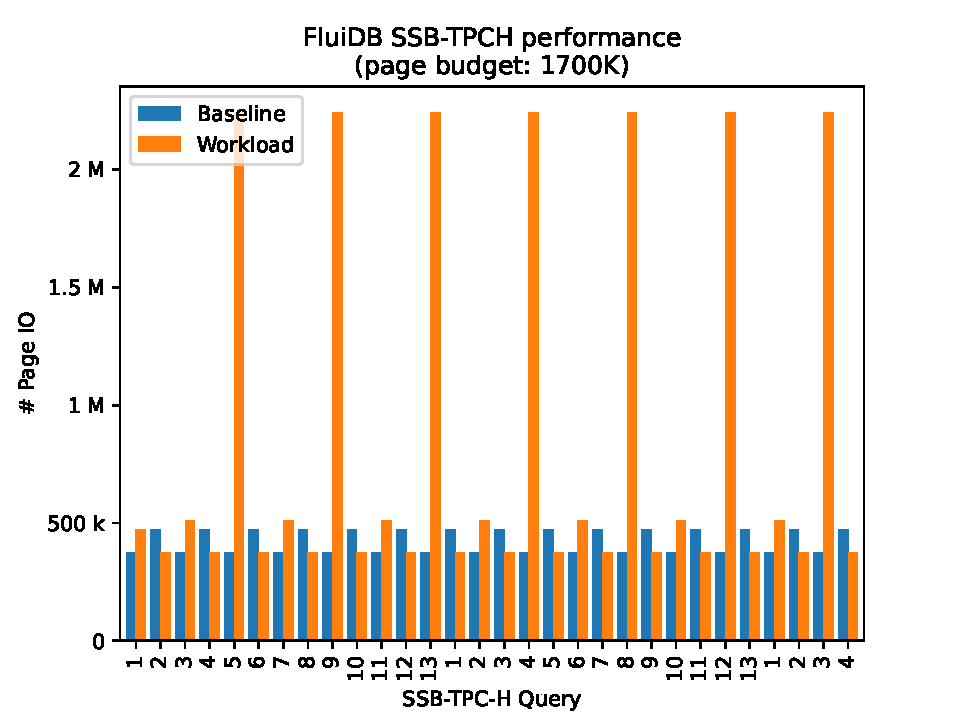
\includegraphics[width=.9\linewidth]{./plans/workload_1700K.pdf}
\caption{\label{fig:gc_enemy}This plot shows a workload where the GC
  opts to remove primary tables in order to make space for
  intermediate results. The primary tables are then required so they
  need to be reconstructed. The general shape of the queries is
  \(A \Join B_0 \Join C_0\) and \(A \Join B_1 \Join C_1\) and the
  budget is small enough that it can't fit the final result, the
  intermediate result and the primary tables simulataneously. The GC
  is therefore required to delete the primary tables forcing their
  reconstruction the next time it is required.}
\end{figure}
\end{correction}


\begin{correction}{Overheads}
  The compilation overheads range between a staggering 9 and 11 secs
  per query. While it is not ideal, there are things that can be done
  to mitigate it like precompiling the headers (eg with the
  \code{-fmodule-header} flag) or changing the granularity of the code
  generation to generate individual operators, which would allow both
  caching of compiled units as well as parallel
  compilation. Optimizing the compilation process itself, however, is
  beyond the scope of this thesis.
\end{correction}


\begin{correction}{Memory budget sensitivity}

\begin{quote}
A sensitivity analysis of the impact of the memory budget –
especially with respect to the role of the garbage collector (GC)
and benefits the proposed system makes even when enough memory is
available and no GC is needed. This will help bring to the fore and
crystalize the benefits of the proposed system.
\end{quote}

It becomes clear from the benchmark results so far that while the GC
often makes the difference between FluiDB being able to successfully
run a query and throwing OOM, and while we have put a lot of care in
tuning it to make good decisions, it can have detrimental effects to
the performance of the sustem as a whole. We can't get away from the
fact that less the GC is triggered, the less likely it is to delete a
query useful in the future.

For that reason, as we discussed in chapter \ref{chapter4} in detail,
FluiDB will only trigger the the GC when it runs out of memory, and
the GC itself goes to great lengths to delete as few tables as
possible. As demonstrated in figure \ref{fig:gc_enemy}, however, the
harsh the memory constraints will casue the GC not only to run more
often it will also be forced to evict relations that are likely to be
necessary for future queries.

While the GC is a central component of FluiDB, the latter is more than
a simple cache system as it involves an advanced planner that can
utilize reversible operations. This means that the search space for
plans is, in principle, larger than the search space that would be
available to a recycling RDBMS that does not take advantage of
reversible operations. As mentioned the performance of FluiDB without
triggering the GC is demonstrated in figure
\ref{fig:extra_large_budget_plot}.
\end{itemize}

\end{correction}

We based our evaluation on the Star Schema Benchmark (SSB)
\cite{barataOverviewDecisionSupport2015} which is a variation of
TPC-H. Like TPC-H it models the data warehouse of a wholesale
supplier.

As the name suggests, these queries query a star schema. The star
schema is derived from the TPC-H schema (figure \ref{fig:tpch_schema})
by merging the \sql{linenumber}, \sql{orders} and
\sql{partsupp} and completely dropped tables \sql{nation} and
\sql{region} tables as shown in figure \ref{fig:ssb_tpch_schema}.

\begin{figure}[p]
\begin{tikzdiagram}
  \tikzset{tbl/.style={draw,rectangle,minimum height=2cm,minimum width=2cm}};
  \node[tbl] (lo) {lineorder};
  \node[tbl] (p) [above left = of lo] {part};
  \node[tbl] (c) [above right = of lo] {customer};
  \node[tbl] (s) [below right = of lo] {supplier};
  \node[tbl] (d) [below left = of lo] {date};
  \draw [-stealth] (c) -- (lo);
  \draw [-stealth] (p) -- (lo);
  \draw [-stealth] (s) -- (lo);
  \draw [-stealth] (d) -- (lo);
\end{tikzdiagram}
\caption{\label{fig:ssb_tpch_schema}The foreign key links in a SSB-TPC-H}
\end{figure}


\begin{figure}[p]
\begin{tikzdiagram}
  \tikzset{tbl/.style={draw,rectangle,minimum height=2cm,minimum width=2cm}};
  \tikzset{arr/.style={-stealth}};
  \node[tbl]                     (r) {region};
  \node[tbl, right=of r]         (n) {nation};
  \node[tbl, above right = of n] (c) {customer};
  \node[tbl, right = of n] (s) {supplier};
  \node[tbl, right = of c]         (o) {orders};
  \node[tbl, right=of s]         (ps) {partsupp};
  \node[tbl, below left = of ps] (p) {part};
  \node[tbl, right= of ps]        (l) {lineitem};
  % Connection
  \path [arr]
  (r) edge (n)
  (n) edge (c)
  (c) edge (o)
  (o) edge (l)
  (n) edge (s)
  (s) edge (ps)
  (ps) edge (l)
  (p) edge (ps);
\end{tikzdiagram}
\caption{\label{fig:tpch_schema}The foreign key links in a traditional TPC-H schema}
\end{figure}


The particular queries contained in the workload are presented in
listing \ref{lst:ssb_sql} in the appendix (\ref{chapter:appendix}).

We generated a workload where queries were compiled and planned one by
one in a loop and were run over a database of data generated with
a modified version of the TPC-H dbgen
\cite{perivolaropoulosFakedrakeSsbdbgen2021a} with scaling of size 1,
meaning that the total primary data totals around 1GB in CSV format. The
exact size of the data generated after formatting them to the format
required by FluiDB (described in chapter \ref{chapter:execution_engine}) are

\begin{minted}[]{sh}
$ du -sh *.dat
4.1M    customer.dat
256K    date.dat
757M    lineorder.dat
31M     part.dat
268K    supplier.dat
\end{minted}

Which makes a total of approximately 200k pages of size 4KB.

\begin{correction}{Exeprimental setup}
  The lowest budget within which FluiDB was able to plan all 13
  queries of SSB-TPC-H was 2300k pages and therefore that was the
  lowest budget we used in our benchmarks. The highest budget we used
  was 6500K pages which is a memory budget that allows the execution
  of all queries without the GC needing to be triggered. Therefore
  FluiDB will have the same performance running our benchmark workload
  for any memory budget over 6500K pages.

  The particulars hardware setup used for the experiment is not
  important for our metrics since, as describe previously, we decided
  that a more useful metric than wall clock time is page IO.
\end{correction}

In our experiment, we use page IO as a proxy for performance, despite
the fact that FluiDB is an in-memory database. We think that this is a
reasonable experimental approach because, as FluiDB leans heavily on
code generation, it is unlikely that the actual instruction retiring
will have a major impact on the performance. Instead, the performance
cost is dominated by page IO that will certainly cause cache misses at
the LLC. Another thing to note is that FluiDB generates code that
focuses on performance and not on compilation time. Making heavy use
of metaprogramming like \cpp{constexpr} makes compilation fairly
slow. There are ways to speed up compilation time like using
pre-compiling header files \cite{PrecompiledHeadersPCH} and
fine-tuning the compiler optimization passes. These techniques are
beyond the scope of this work, FluiDB is focused on analytics
workloads that do not include sub-second queries.

\newcommand{\ioperfdescr}{The total page read/writes for each query of
  SSB TPC-H. The baseline is the query being run by FluiDB directly
  without any materialized n-nodes. The workload bars represent the
  cost of each query in a workload being accumulated into the same
  QDAG. The dashed line represents the performance of sqlite3 with all
  indexes stripped.}
\begin{figure}[H]
\centering
% 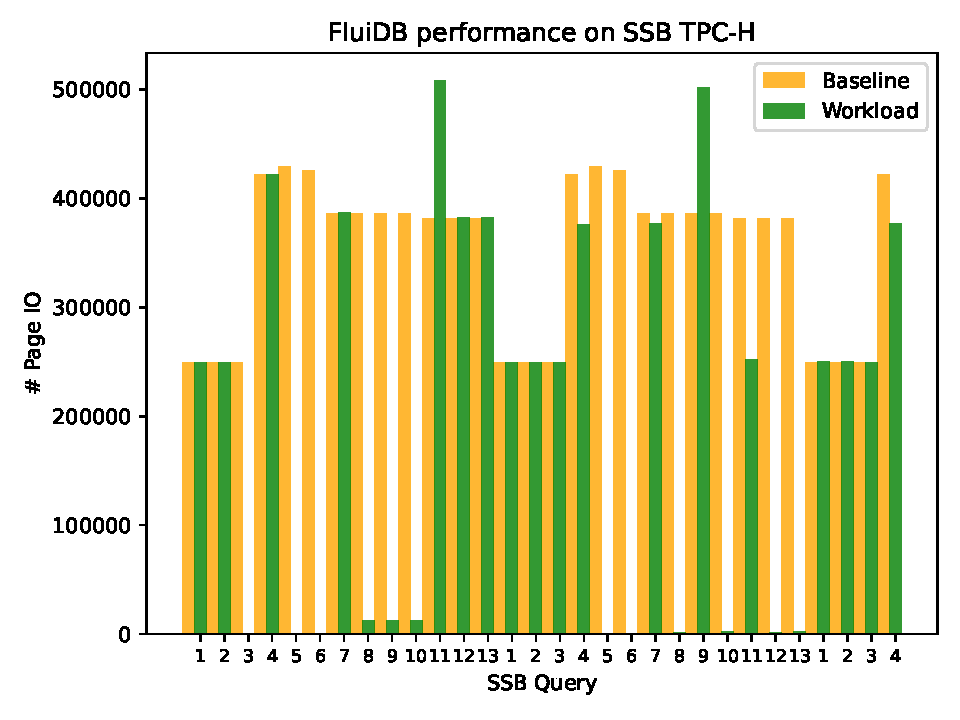
\includegraphics[width=.9\linewidth]{./plans/io_perf_23000.pdf}
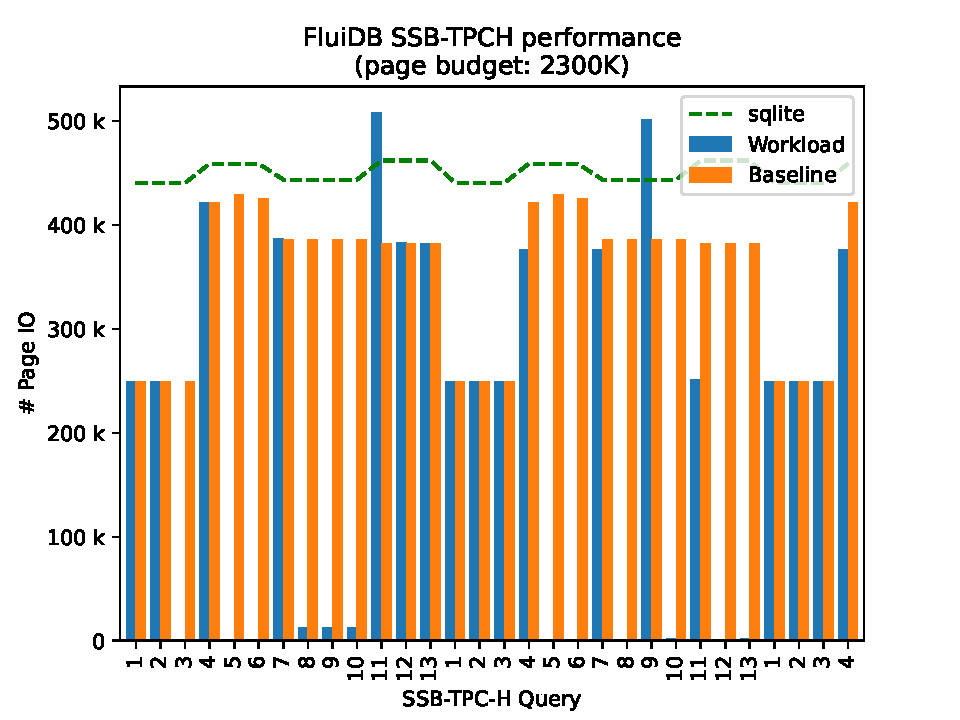
\includegraphics[width=.9\linewidth]{./plans/workload_2300K.pdf}
\caption{\label{fig:min_budget_plot} \ioperfdescr The budget allowed
  for this is the minimum budget within which FluiDB can run each
  individual query (2300K pages).}
\end{figure}

Figure \ref{fig:min_budget_plot} demonstrates that FluiDB running a
workload versus running each query individually causes speedups even
in constrained budgets. This particular run is run on the minimum
space budget for which the planner is able to create plans for every
individual query. In some cases, however, the garbage collector is
forced to delete tables that need to be recreated later in the
workload causing FluiDB to be sporadically less performant than the
base case.

For a larger budget, the FluiDB is able to store more useful
intermediate results as demonstrated in figure
\ref{fig:large_budget_plot}.

\begin{figure}[H]
\centering
%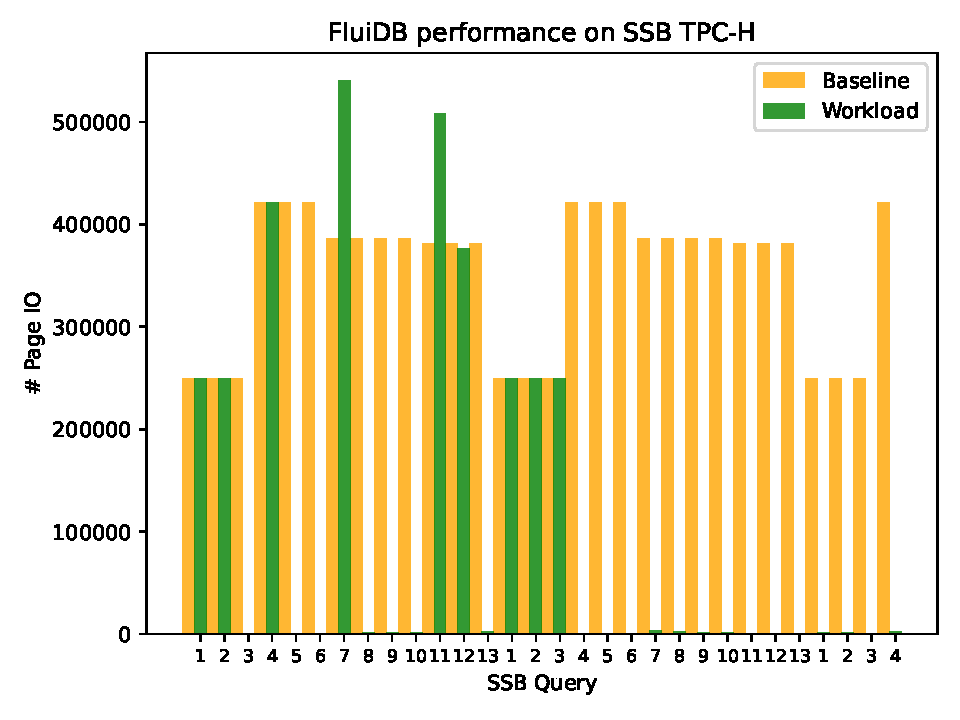
\includegraphics[width=.9\linewidth]{./plans/io_perf_61000.pdf}
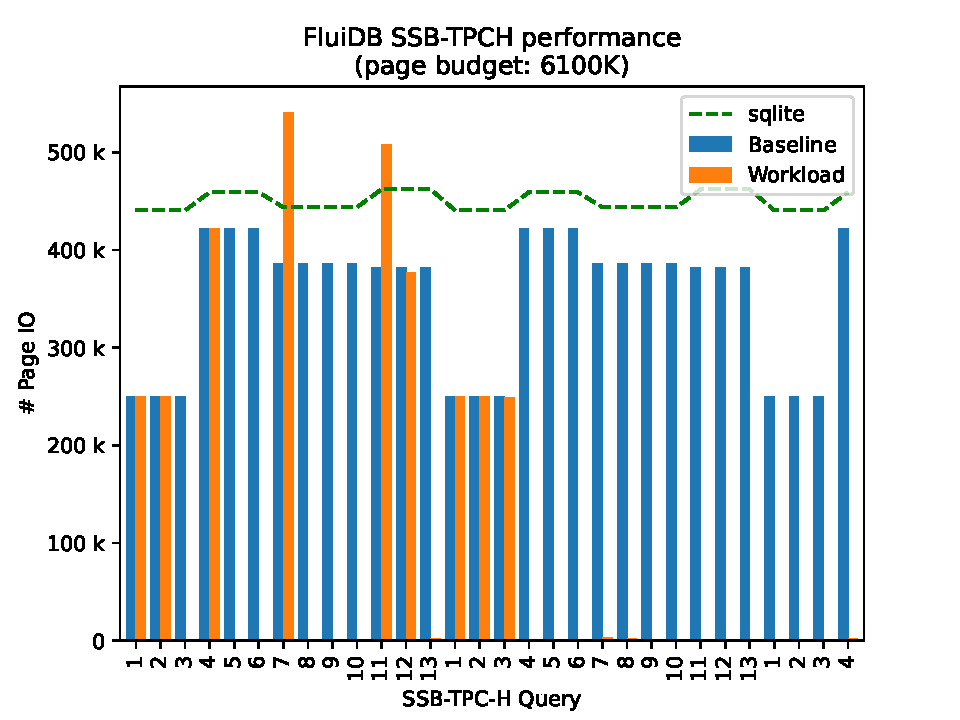
\includegraphics[width=.9\linewidth]{./plans/workload_6100K.pdf}
\caption{\label{fig:large_budget_plot} \ioperfdescr The budget
  allowed for this is about triple the minimum budget within which
  FluiDB can run each individual query (6100K pages). A badly timed GC
  run causes some individual queries to be slower than their
  counterparts from a workload being run in a tight budget (figure
  \ref{fig:min_budget_plot}).}
\end{figure}

An interesting point here is the plan for evaluating query 7 is more
expensive in the workload run under laxer budgetary constraints. This
may seem strange but it is an example demonstrative of the fundamental
operation of FluiDB. The high level explanation for this is that the
high-budget plan needs to evaluate \(\mathit{lineorder}\) via the
reverse trigger of a join as it was deleted during the evaluation of
query 6. Mysteriously, during the strict-budget planning the
\(\mathit{lineorder}\) relation is readily available during the
planning of query 7! The key lies slightly earlier in the workload
(see listing \ref{fig:reverse_operations}).

FluiDB materializes in query 4 the join

\[
Q_{36} := \mathit{supplier} \Join_{\mathit{lo\_suppkey} = \mathit{s\_suppkey}} \mathit{lineorder}
\]

and the corresponding antijoins \(Q_{35}\) and \(Q_{37}\), making the
node \(\mathit{lineorder}\) deletable. However, when running the
workload under strict budgetary constraints, it is forced to garbage
collect shortly after materializing said join at a moment while both
\(Q_{36}\) and \(\mathit{lineorder}\) are protected (see section
\ref{sec:gc} on garbage collection). Therefore, FluiDB is forced to
delete both \(Q_{35}\) and \(Q_{37}\), making \(\mathit{lineorder}\)
non-deletable when planning for query 4 finishes.

On the other hand, with laxer budgetary constraints, no garbage
collection is triggered during query 4. The next garbage collection is
triggered during query 6, at a moment when \(\mathit{lineorder}\) is
deletable, unprotected, and a prime candidate for deletion based on
the GC heuristics. nnAlas, when query 7 requires \(\mathit{lineorder}\)
for its plan, FluiDB needs to reconstruct it in the case of lax
budgetary constraints but not in the case of strict constraints.

This example of FluiDB being forced to locally produce more expensive
plans is an effect of FluiDB being more opportunistic, the lower the
available budget is, and more adventurous when operating with high
budgets. When FluiDB is frugal, it is generally prone to miss
opportunities to share computation between queries. There are times
however that this frugality saves it from bad heuristic-based
decisions that it is allowed to make otherwise.

\begin{code}
\begin{minted}[escapeinside=||,mathescape=true]{trace-lexer.py:TraceLexer -x}
# Query 4
Query |\(s \gamma \pi \sigma (\mathit{supplier} \Join \mathit{lineorder} \Join \mathit{date} \Join \mathit{part})\)| {
  # There is enough space to keep both and the complements
  |\(Q_{36}, Q_{35}, Q_{37}\)| := Materialize[|\(\mathit{supplier} \Join \mathit{lineorder}, \mathit{supplier} \cancel\ltimes \mathit{lineorder}, \mathit{supplier} \cancel\rtimes \mathit{lineorder}\)|]
  |\(Q_{41}, Q_{40}, Q_{42}\)| := Materialize[|\(Q_{36} \Join \mathit{date}, Q_{36} \cancel\ltimes \mathit{date}, Q_{36} \cancel\rtimes \mathit{date}\)|]
  |\(Q_{46}, Q_{45}, Q_{47}\)| := Materialize[|\(Q_{41} \Join \mathit{part}, Q_{41} \cancel\ltimes \mathit{part}, Q_{41} \cancel\rtimes \mathit{part}\)|]
  |\(Q_{50}\)| := Materialize[|\(\sigma Q_{46}\)|]
  |\(Q_{90}\)| := Materialize[|\(\gamma \pi Q_{50}\)|]
  |\(Q_{91}\)| := Materialize[|\(s Q_{90}\)|]
}

# Query 5
Query |\(s \gamma \pi \sigma (\mathit{supplier} \Join \mathit{lineorder} \Join \mathit{date} \Join \mathit{part})\)| {
  |\(Q_{92}\)| := Materialize[|\(\sigma Q_{46}\)|]
  |\(Q_{118}\)| := Materialize[|\(\gamma \pi Q_{92}\)|]
  |\(Q_{119}\)| := Materialize[|\(s Q_{118}\)|]
}

# Query 6
Query |\(s \gamma \pi \sigma (\mathit{supplier} \Join \mathit{lineorder} \Join \mathit{date} \Join \mathit{part}))\)| {
  # FluiDB decides delete lineorder since it has the complements
  GC { Delete[|\(\ldots, \mathit{lineorder}, \ldots \)|] }
  |\(Q_{120}\)| := Materialize[|\(\sigma Q_{46}\)|]
  |\(Q_{146}\)| := Materialize[|\(\gamma \pi Q_{120}\)|]
  |\(Q_{147}\)| := Materialize[|\(s Q_{146}\)|]
}

# Query 7
Query |\(s \gamma \pi \sigma (\mathit{customer} \Join \mathit{date} \Join \mathit{lineorder} \Join \mathit{supplier})\)| {
  # Ooops... this would be avoided if we hadn't deleted lineorder.
  |\(\mathit{lineorder}\)| := Materialize[|\(\bar\pi Q_{36} \cup Q_{37}\)|]
  |\(\mathit{date}\)| := Materialize[|\(\bar\pi Q_{41} \cup Q_{42}\)|]
  GC { Delete[|\( \ldots \)|] }
  |\(Q_{149}, Q_{148}, Q_{150}\)| := Materialize[|\(\mathit{date} \Join \mathit{lineorder}, \mathit{date} \cancel\ltimes \mathit{lineorder}, \mathit{date} \cancel\rtimes \mathit{lineorder}\)|]
  GC { Delete[|\( \ldots \)|] }
  |\(Q_{154}, Q_{153}, Q_{155}\)| := Materialize[|\(\mathit{customer} \Join Q_{149}, \mathit{customer} \cancel\ltimes Q_{149}, \mathit{customer} \cancel\rtimes Q_{149}\)|]
  GC { Delete[|\( \ldots \)|] }
  |\(Q_{165}\)| := Materialize[|\(\sigma Q_{154}\)|]
  |\(Q_{182}, Q_{181}, Q_{183}\)| := Materialize[|\(Q_{165} \Join \mathit{supplier}, Q_{165} \cancel\ltimes \mathit{supplier}, Q_{165} \cancel\rtimes \mathit{supplier}\)|]
  GC { Delete[|\( \ldots \)|] }
  |\(Q_{163}\)| := Materialize[|\(\sigma Q_{182}\)|]
  |\(Q_{203}\)| := Materialize[|\(\gamma \pi Q_{163}\)|]
  |\(Q_{204}\)| := Materialize[|\(s Q_{203}\)|]
}

\end{minted}
  \caption{\label{fig:reverse_operations}Abbreviated version of the
    plans of queries 4 to 7 of SSB TPC-H. This demonstrates how an
    unfortunately timed GC can cause cause FluiDB to make some bad decisions}

\end{code}

FluiDB aspires to deal with the entire workload as if it were planning
a single query. While any decision during the planning of a single
query can be scrapped in the backtracking process, FluiDB is
tragically forced to commit to whatever adventurous or conservative
decisions it makes at the end of every planning iteration, doomed to
pay dearly for every misstep but to reap the rewards of every
insightful choice.

Interestingly, this problem goes away when we run with a budget of
3500k pages (figure \ref{fig:extra_large_budget_plot}) as the GC run
is delayed to a time when other relations are better candidates for
deletion than \(\mathit{lineorder}\). A carefully designed set of
heuristics for the GC should avoid this problem in most cases.

\begin{figure}[p]
\centering
% 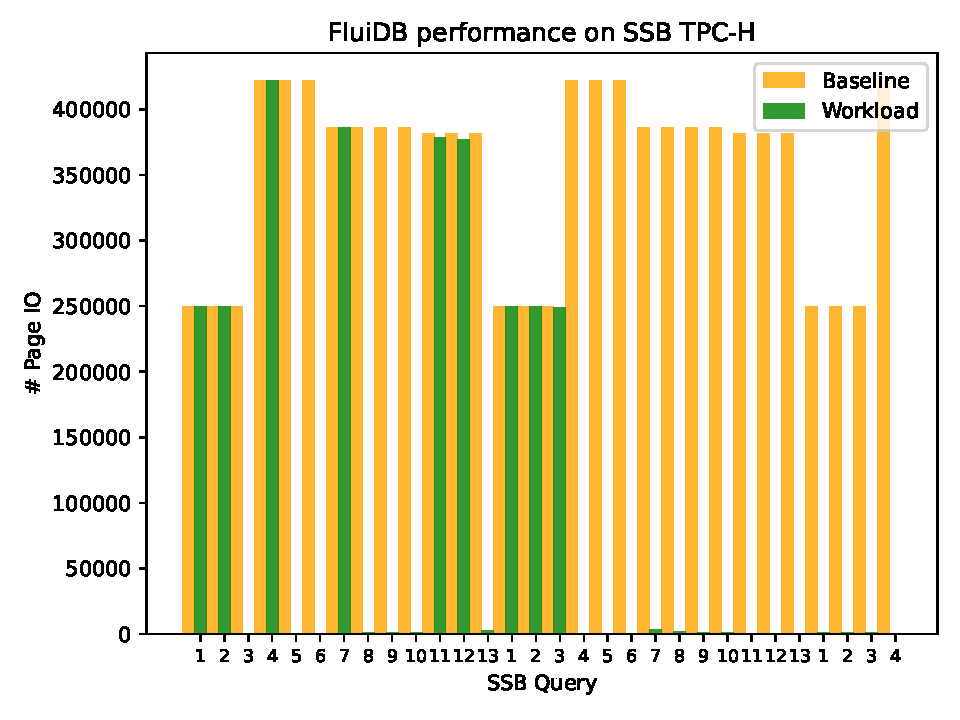
\includegraphics[width=.9\linewidth]{./plans/io_perf_65000.pdf}
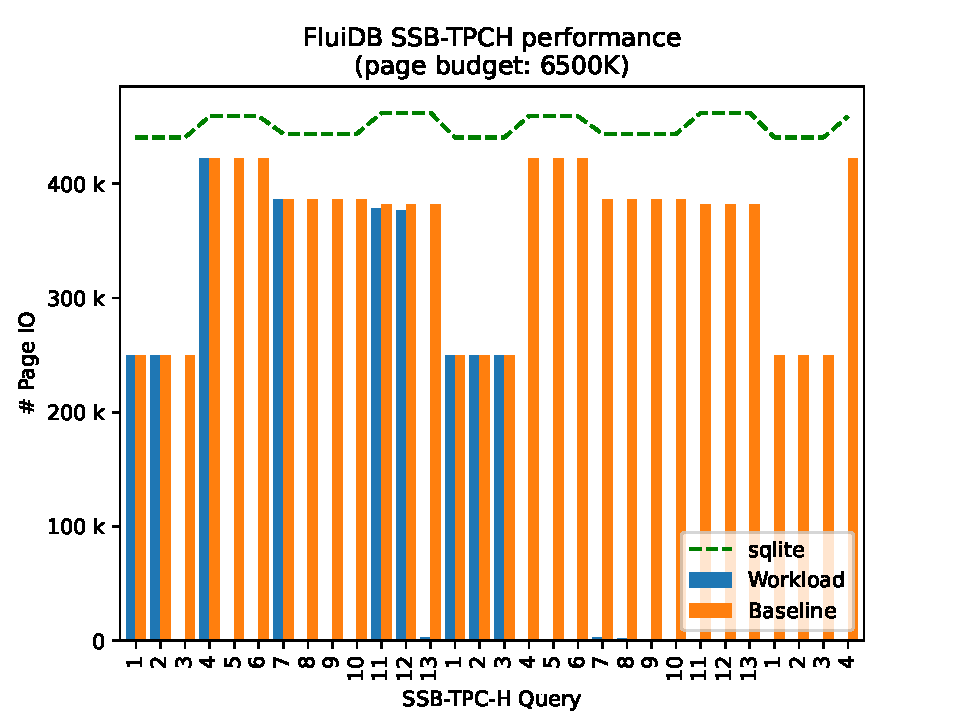
\includegraphics[width=.9\linewidth]{./plans/workload_6500K.pdf}
\caption{\label{fig:extra_large_budget_plot}
\ioperfdescr. The budget
  allowed for this is about triple the minimum budget within which
  FluiDB can run each individual query (6500K pages).}
\end{figure}

\begin{comment}
\section{A note on size estimation}
\label{sec:size_estimation_problems}
The size of the budget may seem fairly excessive for the size required
for the primary tables. To understand why that is, we need to look at
the largest n-nodes in the QDAG:

\begin{center}
\begin{tabular}{rl}
Pages & Expr\\
\hline
188000 & \(lineorder\)\\
547100 & \(customer \Join (date \Join lineorder)\)\\
376200 & \(\sigma ((customer \Join (date \Join lineorder)) \Join supplier)\)\\
376200 & \(\sigma ((date \Join lineorder)) \Join supplier)\)\\
273600 & \(\sigma (customer \Join (date \Join lineorder))\)\\
188100 & \(\sigma ((\sigma (customer \Join (date \Join lineorder))) \Join supplier)\)\\
\end{tabular}
\end{center}

From looking at those n-nodes it seems that a sufficiently advanced
garbage collector should be able to support plans that materialize the
n-nodes in about half the budget as FluiDB should have been able to plan
the query needing around double the pages required to store the largest equijoin
which for us is \(customer\) date \(lineorder\).

The main issue, however, as it is with many query processing systems
\cite{leisHowGoodAre2015}, is the cardinality estimator which assumes
that in a natural join there are no foreign key lookup failures, that
is, that all natural joins are extension joins. Therefore

\[
\lvert \sigma _{p(customer)} (customer \Join (date \Join lineorder)) \rvert = \lvert (\sigma _{p(customer)} customer \Join (date \Join lineorder)) \rvert
\]


This causes FluiDB to vastly overestimate the size of plans that have
selections pushed down, making these plans disproportionately
unappealing.
\end{comment}

\section{Conclusion}

FluiDB is a complex database system built from scratch focused on a
specific idea: making optimal use of the storage budget by fully
adapting the data layout to the workload. While FluiDB is an
experimental system that is probably not stable enough system to be
used in a production setting, it is a complete end-to-end system and
the results presented in this chapter demonstrate that it is based on
ideas worth considering in the design of a commercial database system.


\chapter{Conclusions and future perspectives}
\label{chapter:conclusion}
TODO


\appendix
\chapter{Appendix}
\label{chapter:appendix}
\todo{describe ListT and refer to it}
\begin{code}
\inputminted{text}{./plans/low_budget.plan}
\caption{\label{fig:workload_plans}
  The query plans emitted for the minimum size workload}
\end{code}

\begin{code}
\inputminted{text}{./plans/baseline.plan}
\caption{\label{lst:baseline_plans}The query plans emitted for baseline queries}
\end{code}

\begin{code}
\inputminted{text}{./plans/ssb_queries.sql}
\caption{\label{fig:ssb_sql}The SQL code for the 12 SSB queries}
\end{code}


% single spacing for bibliography
\begin{spacing}{1}
\printbibliography
\end{spacing}

\backmatter

\end{document}
